%%%%%%%%%%%%%%%%%%%%%%%%%%%%%%%%%%%%%%%%%%%%%%%%%%%%%%%%%%%%%%%%%%%%%%%
\chapter{Multi-body Systems}
\label{ch:multibody}
%%%%%%%%%%%%%%%%%%%%%%%%%%%%%%%%%%%%%%%%%%%%%%%%%%%%%%%%%%%%%%%%%%%%%%%



Extending bond graph modelling from 2D plane motion to full \textbf{3D rigid-body mechanics} brings geometric nonlinearity through the rotation group. These geometric nonlinearities are a primary cause of equation formulation problems. The key modelling choice — whether to express quantities in the inertial frame or a body-fixed frame — has direct consequences for the structure of the equations and the bond graph.

\section{Dynamics of a 3D rigid body}

Consider a rigid body of mass $m$ with moments of inertia $J_x, J_y, J_z$ along the principal axes. The body-fixed coordinate frame $\{G; x, y, z\}$ is attached to the center of mass $G$ with axes aligned with the principal axes of inertia. 

\paragraph{Why the body frame?}
In the inertial frame, the inertia tensor $\mathbf{J}$ is a $3\times3$ matrix that varies with the body's orientation — making the constitutive equations of the I-field time-varying and complex. In the body frame, $\mathbf{J} = \mathrm{diag}(J_x, J_y, J_z)$ is \textbf{constant}, which is the primary advantage of this formulation. The mass $m$ and inertia $\mathbf{J}$ are invariant, making them highly practical coordinates for computation.

The price is that Newton's law in the body frame contains \textbf{nonlinear gyroscopic terms} from the frame's own rotation. Newton's law applied in the body frame requires accounting for the rate of change of momentum relative to the moving frame.

\paragraph{Newton--Euler equations.}
Let $\mathbf{v} = (v_x, v_y, v_z)^T$ and $\boldsymbol{\omega} = (\omega_x, \omega_y, \omega_z)^T$ be the translational velocity of $G$ and the angular velocity, \emph{both expressed in the body frame}. Let $\mathbf{F}$ and $\boldsymbol{\tau}$ be force and torque at $G$ in the body frame. Then:
\begin{equation}
  \mathbf{F} = \dot{\mathbf{p}} + \boldsymbol{\omega}\times\mathbf{p},
  \qquad \mathbf{p} = m\mathbf{v},
\end{equation}
\begin{equation}
  \boldsymbol{\tau} = \dot{\mathbf{h}} + \boldsymbol{\omega}\times\mathbf{h},
  \qquad \mathbf{h} = \mathbf{J}\boldsymbol{\omega}.
\end{equation}
Written component-wise, these are the \textbf{Euler equations}:
\begin{align}
  F_x &= m\dot{v}_x + m\omega_y v_z - m\omega_z v_y \notag\\
  F_y &= m\dot{v}_y + m\omega_z v_x - m\omega_x v_z \notag\\
  F_z &= m\dot{v}_z + m\omega_x v_y - m\omega_y v_x \notag\\[4pt]
  \tau_x &= J_x\dot{\omega}_x + \omega_y J_z\omega_z - \omega_z J_y\omega_y \notag\\
  \tau_y &= J_y\dot{\omega}_y + \omega_z J_x\omega_x - \omega_x J_z\omega_z \notag\\
  \tau_z &= J_z\dot{\omega}_z + \omega_x J_y\omega_y - \omega_y J_x\omega_x.
\end{align}


\begin{insightbox}
  Note that we are dealing the body fixed frame here. This is just the derivative wrt to time of a vector, that in this case are the momentum ($p$) and the angular momentum ($h$). There is a \textbf{hidden frame fixed to the momentum vectors.} 

  The angular momentum formula is more intuitive since it's more used as we work with fixed body frame with fixed inertia and axis of inertia. This is not usually done with forces, since we see them in the inertial frame. 

  Note also that it's always possible to measure $\omega$ with a gyro, since all the points in a rigid body have the same angular velocity. However, the linear velocity of the CoG is not directly measurable by a sensor fixed to the body, since it depends on the point itself. That's why we don't use the first equations in practice.

  \begin{figure} [H]
    \centering
    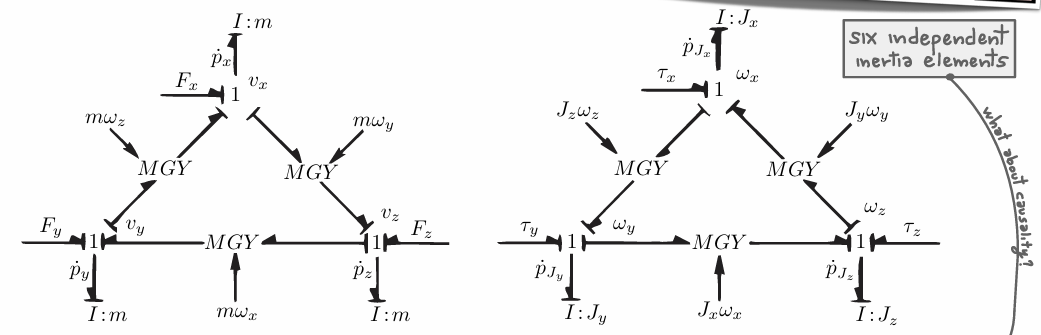
\includegraphics[width=0.8\textwidth]{figs/chapter6/6_1.png}
    \caption{Considerations on the body frame and the hidden frame of the momentum vectors.}
  \end{figure}

\end{insightbox}



These nonlinear differential equations have no general analytical solution. Furthermore, they provide velocities with respect to a frame that is aiming in a different direction at every instant. The cross-product terms $\boldsymbol{\omega}\times\mathbf{p}$ and $\boldsymbol{\omega}\times\mathbf{h}$ are gyroscopic: they do not do work (they are perpendicular to velocity), but they redistribute momentum between components. In the bond graph, they appear as \textbf{modulated gyrators} (MGY elements) whose moduli depend on the angular velocity — making the model intrinsically nonlinear.

\begin{insightbox}[The I-field of a 3D rigid body vs. Independent Elements]
The 3D rigid body is conceptually represented by a \textbf{6-port I-field} in the body frame: three translational ports and three rotational ports. The constitutive law (flow = $\mathbf{M}^{-1}\mathbf{p}$, with block-diagonal $\mathbf{M} = \mathrm{diag}(m\mathbf{I}_3, \mathbf{J})$) is linear and constant. 

However, \emph{attention must be paid to the actual bond graph implementation}. In practice, this block is modelled as \textbf{six independent 1-port I-elements}, which are in integral causality. (since the mass matrix is diagonal in the principal body frame), interconnected by an Eulerian junction structure containing the MGYs. The nonlinear gyroscopic interaction is handled by MGY elements in the junction structure, not inside the I-elements themselves. This separation of linear storage from nonlinear routing is elegant and computationally efficient. As long as external forces and torques are causal inputs, integral causality exists for all six I-elements.
\end{insightbox}

\begin{figure} [H]
  \centering
  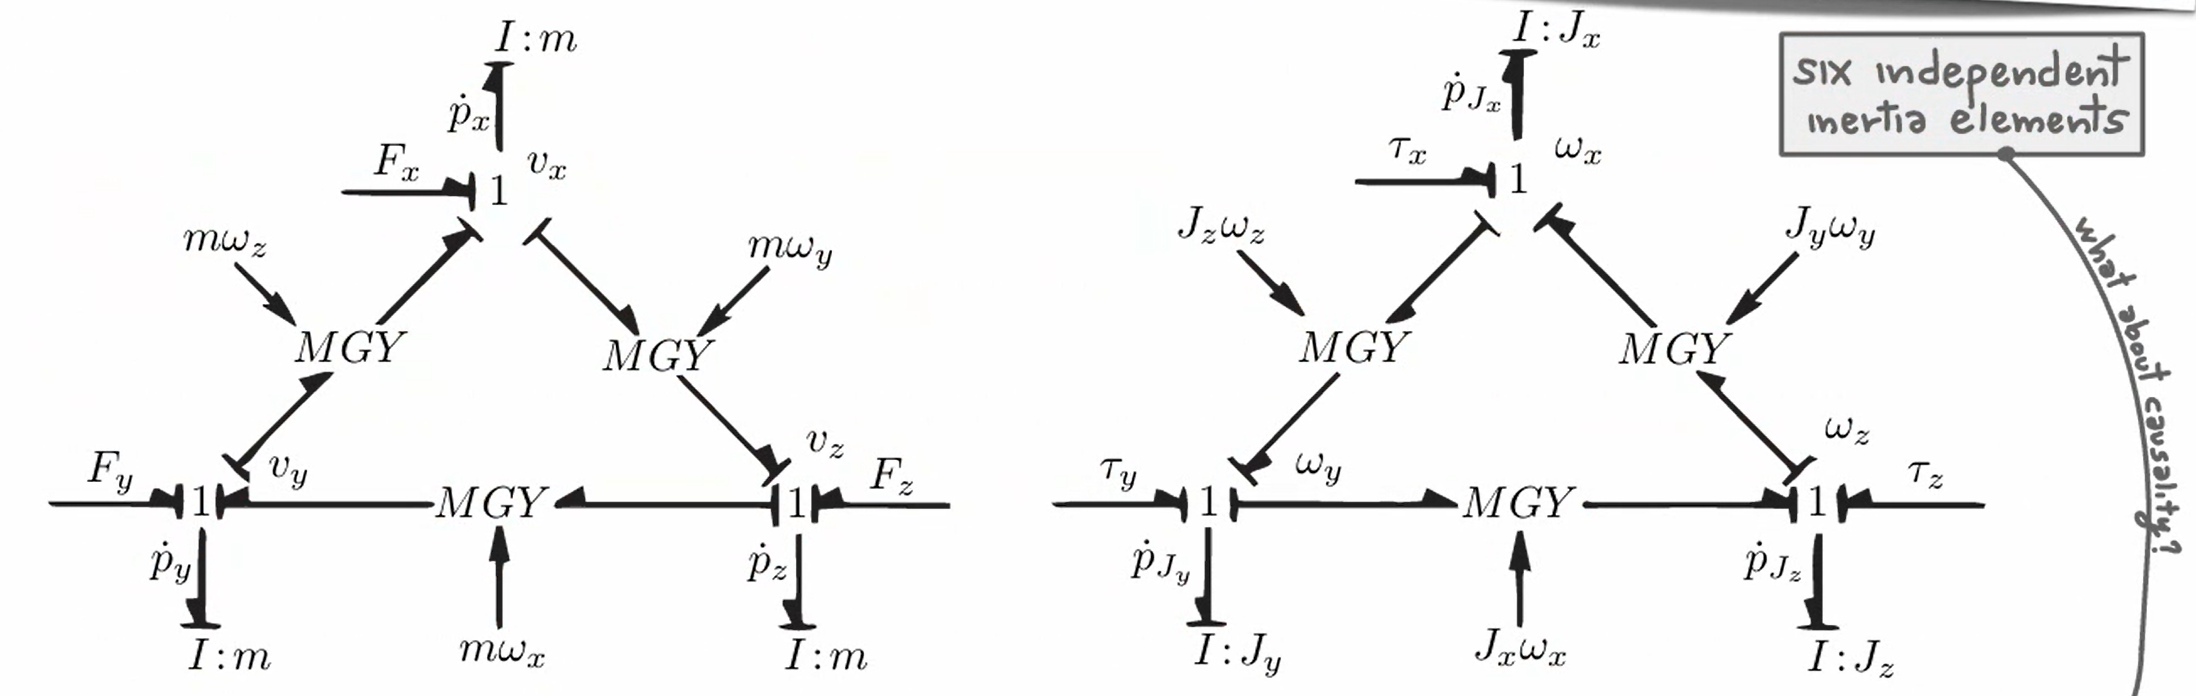
\includegraphics[width=0.8\textwidth]{figs/chapter6/6_2.png}
  \caption{The I-field of a 3D rigid body is often implemented as six independent I-elements (three for translation, three for rotation) interconnected by a junction structure that encodes the gyroscopic interactions via MGY elements.}   
\end{figure}

\begin{figure}
  \centering
  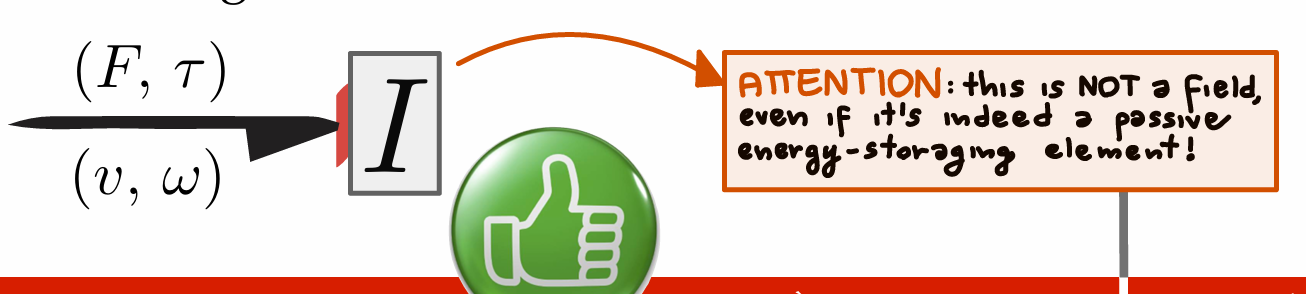
\includegraphics[width=0.8\textwidth]{figs/chapter6/6_2_1.png}
  \caption{THis is not a single field, this is a double field because they are two separated systems.}
\end{figure}

Note that in the bond enters the ($F_x, _y, F_z$) forces that's important to mention that they are refered to the body frame (which is moving w.r.t. the inertial frame). Forces assign causality effort, and the I-field is in integral causality, so the velocities are outputs. The MGY elements take these velocities and feed them back into the I-field to account for the gyroscopic effects.

\section{Rotation matrices and coordinate transformations}

Since all velocities and forces are expressed in the body frame, but external loads and gravity often come from the inertial frame (where e.g., gravity acts strictly downwards), coordinate transformations are necessary. We need an appropriate "junction element" to bridge the body frame and the inertial frame.

The rotation matrix $\mathbf{R}(t)$ (a $3\times3$ orthogonal matrix with $\mathbf{R}^T\mathbf{R} = \mathbf{I}$, $\det\mathbf{R} = 1$) transforms vectors from the body frame to the inertial frame ($\mathbf{w}_{inertial} = \mathbf{R} \mathbf{w}_{body}$). In bond graphs, $\mathbf{R}$ acts as a Modulated Transformer (MTF) that conserves power.

\paragraph{Yaw, Pitch, and Roll (Cardan Angles).}
Any spatial transformation consists of a series of coordinate rotations. For spinning bodies, Euler angles are typical, but for multi-body systems like robotic arms or aircraft, Yaw ($\psi$), Pitch ($\theta$), and Roll ($\phi$) (Cardan Angles) are frequently used. The combined rotation matrix is $\mathbf{R}_{\psi\theta\phi} = \mathbf{R}_\psi \mathbf{R}_\theta \mathbf{R}_\phi$.

By mapping the body-frame angular velocity $\boldsymbol{\omega}$ to the angle derivatives, we obtain the kinematic relationships:
\begin{align}
  \dot{\psi} &= \frac{\sin\phi}{\cos\theta}\omega_y + \frac{\cos\phi}{\cos\theta}\omega_z \\
  \dot{\theta} &= \cos\phi\, \omega_y - \sin\phi\, \omega_z \\
  \dot{\phi} &= \omega_x + \sin\phi\frac{\sin\theta}{\cos\theta}\omega_y + \cos\phi\frac{\sin\theta}{\cos\theta}\omega_z
\end{align}

\begin{figure} [H]
  \centering
  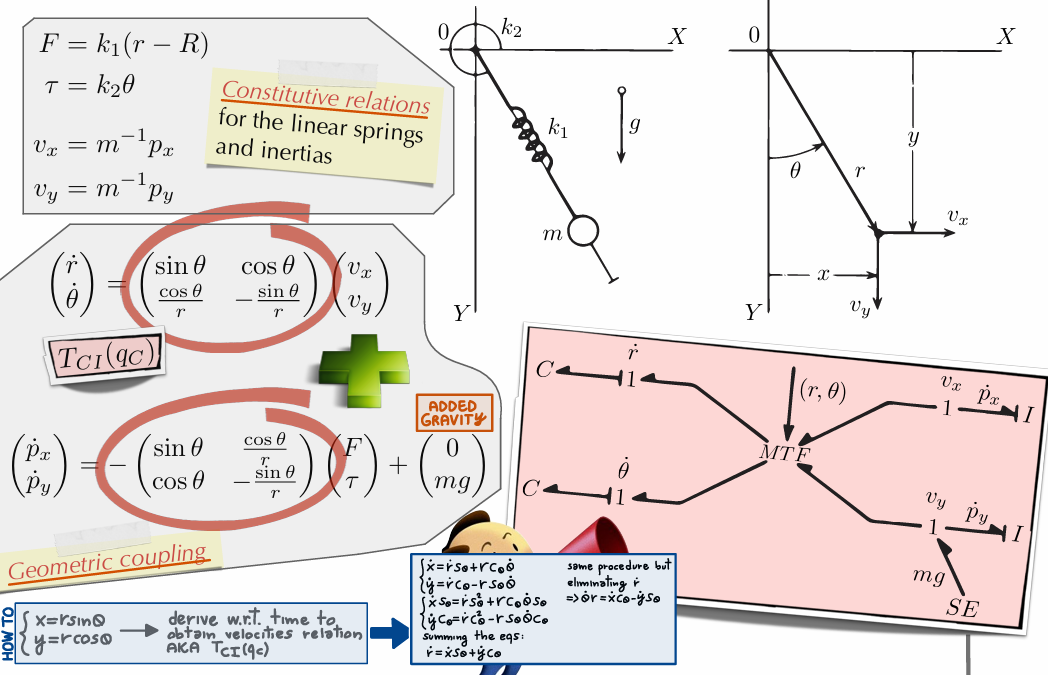
\includegraphics[width=0.8\textwidth]{figs/chapter6/6_3.png}
  \caption{Roll pitch and yaw rotation matrices}  
\end{figure}


Care must be taken regarding kinematic singularities (e.g., when $\cos\theta = 0$). Alternatively, one can directly integrate the differential equation of the rotation matrix:
\begin{equation}
  \dot{\mathbf{R}} = \mathbf{R}\,\mathbf{S}(\boldsymbol{\omega})
\end{equation}
where $\mathbf{S}(\boldsymbol{\omega})$ is the skew-symmetric matrix:
\begin{equation}
  \mathbf{S}(\boldsymbol{\omega}) = \begin{pmatrix}0 & -\omega_z & \omega_y\\\omega_z & 0 & -\omega_x\\-\omega_y & \omega_x & 0\end{pmatrix}.
\end{equation}
The quantity $\dot{\mathbf{R}}\mathbf{R}^T = \mathbf{R}\,\mathbf{S}(\boldsymbol{\omega})\,\mathbf{R}^T$ is the angular velocity in the inertial frame expressed as a skew-symmetric matrix. In the bond graph, MTF elements with moduli from $\mathbf{R}$ handle these transformations when coupling to the environment or to other bodies.

\begin{figure} [H]
  \centering
  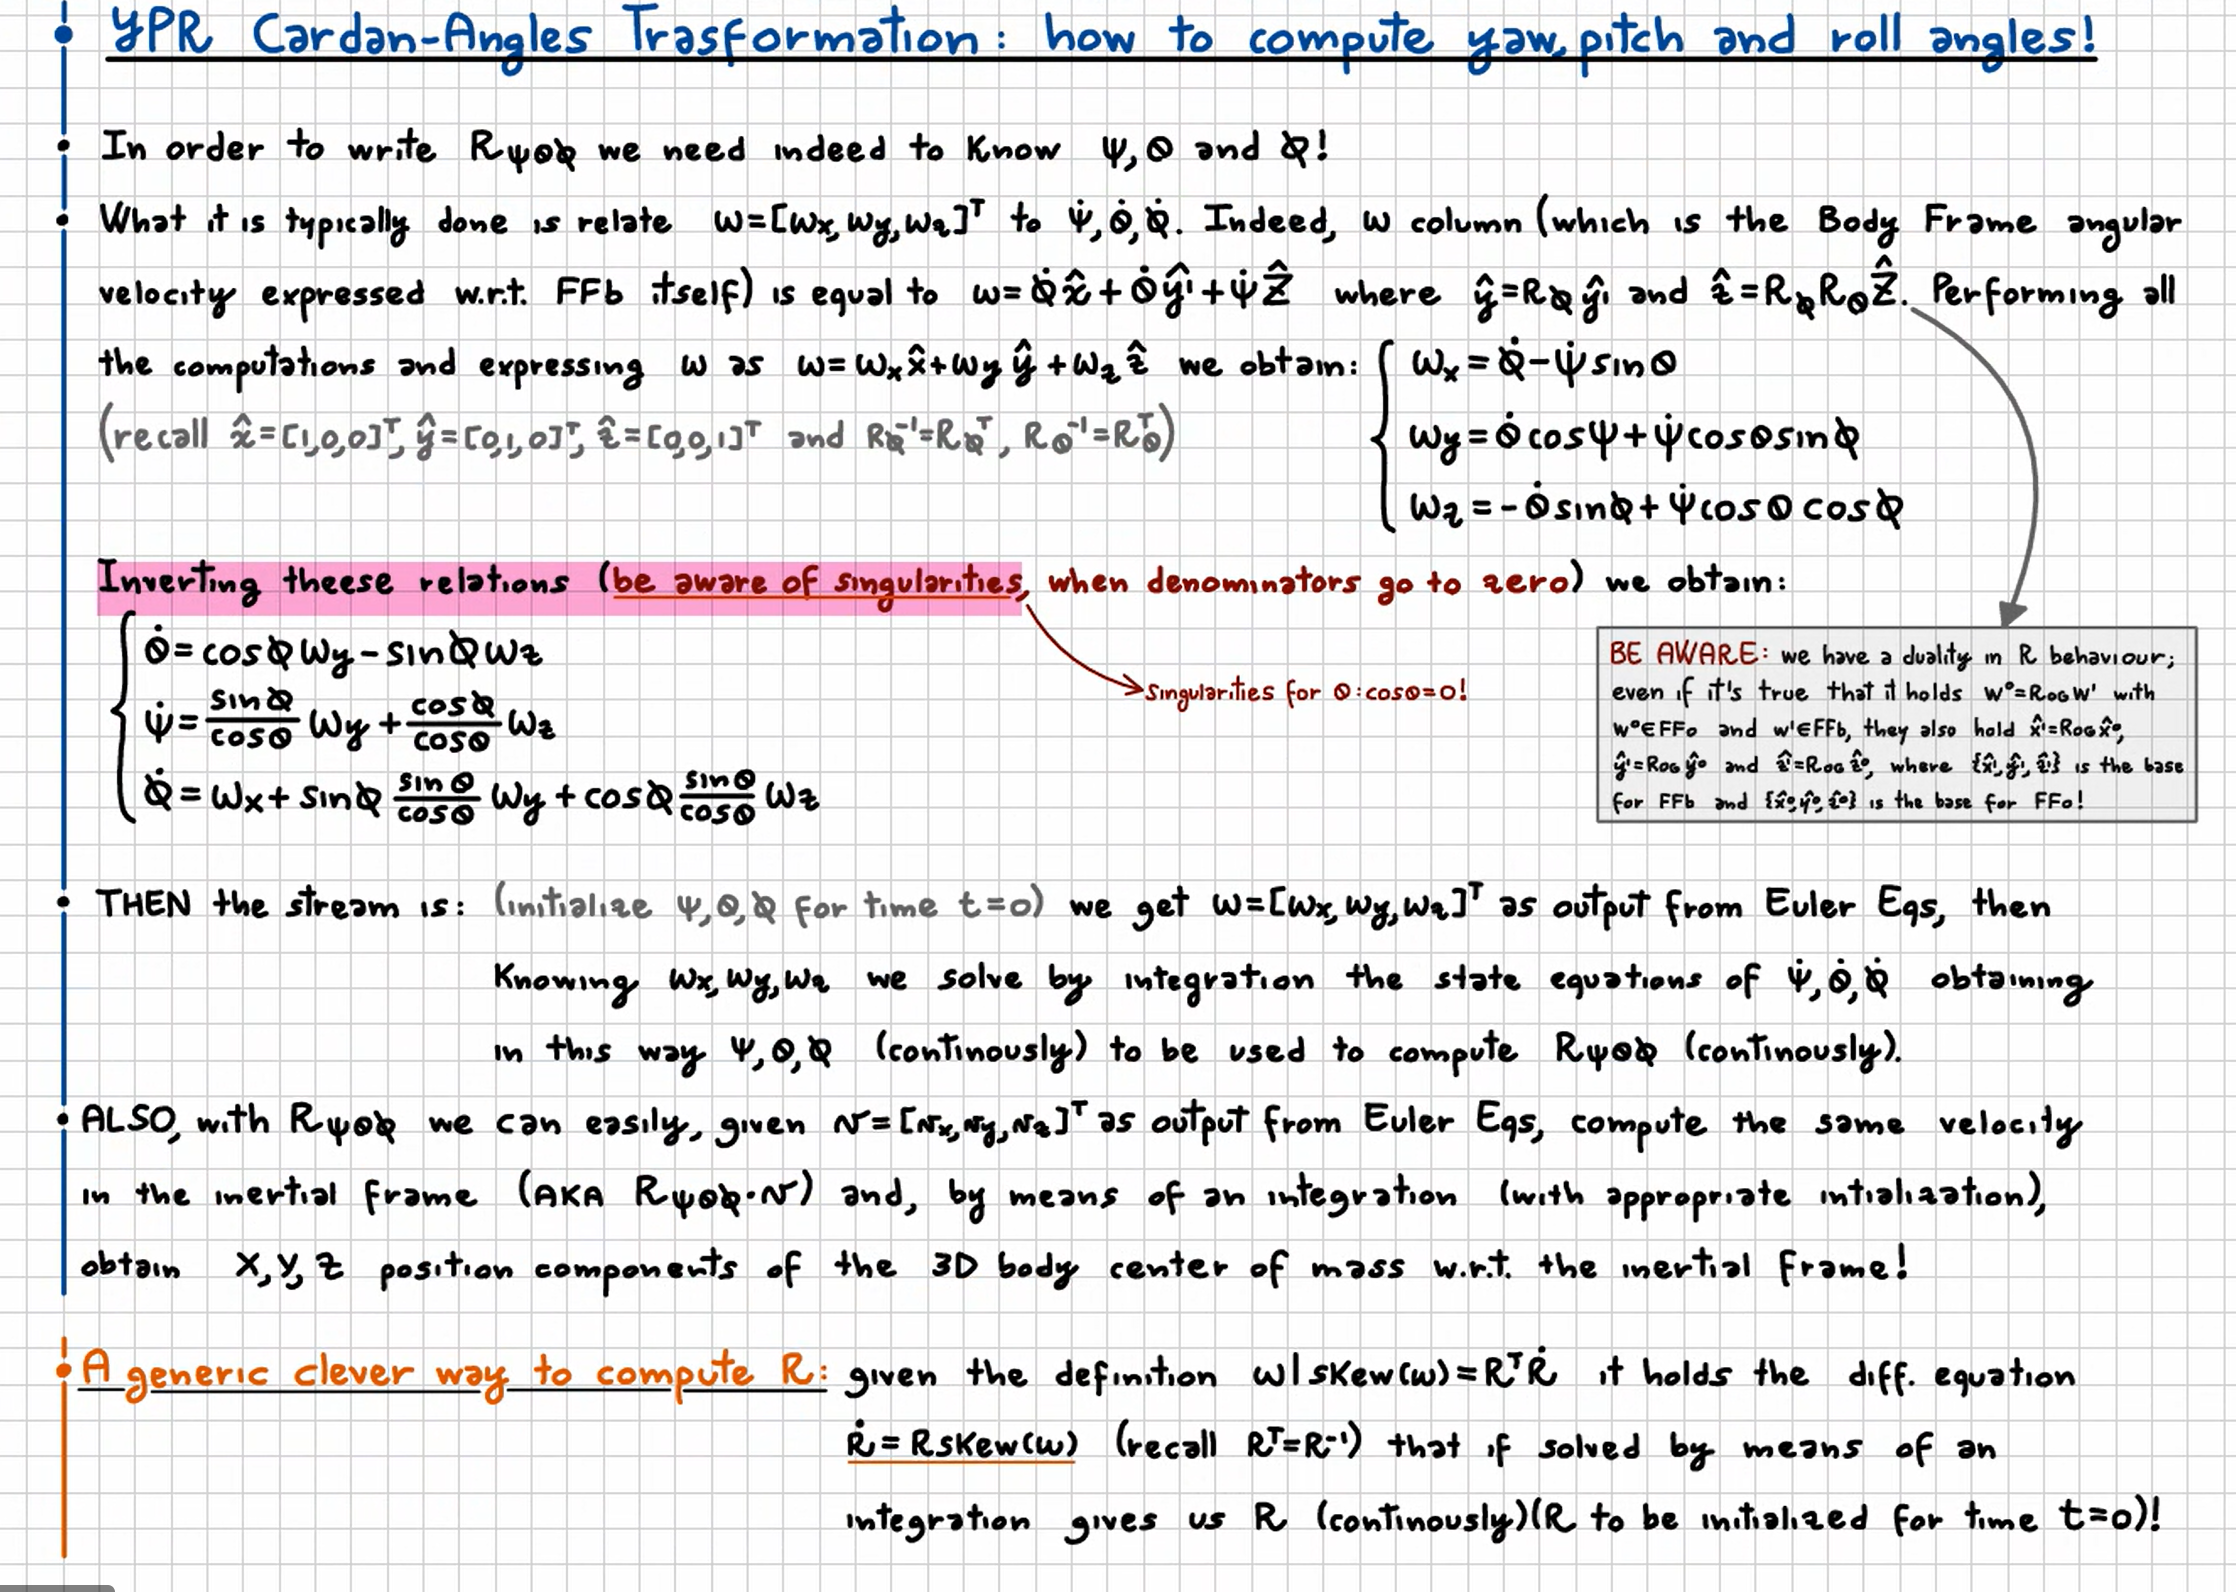
\includegraphics[width=0.8\textwidth]{figs/chapter6/6_4.png}
  \caption{Andrea Lombardi insight}
\end{figure}


\paragraph{Multidimensional dynamics}

We can always tranform the body-fixed variables into inertial frame variables by using a modulated transformer that handles the rotation. 

\begin{figure}[H]
  \centering
  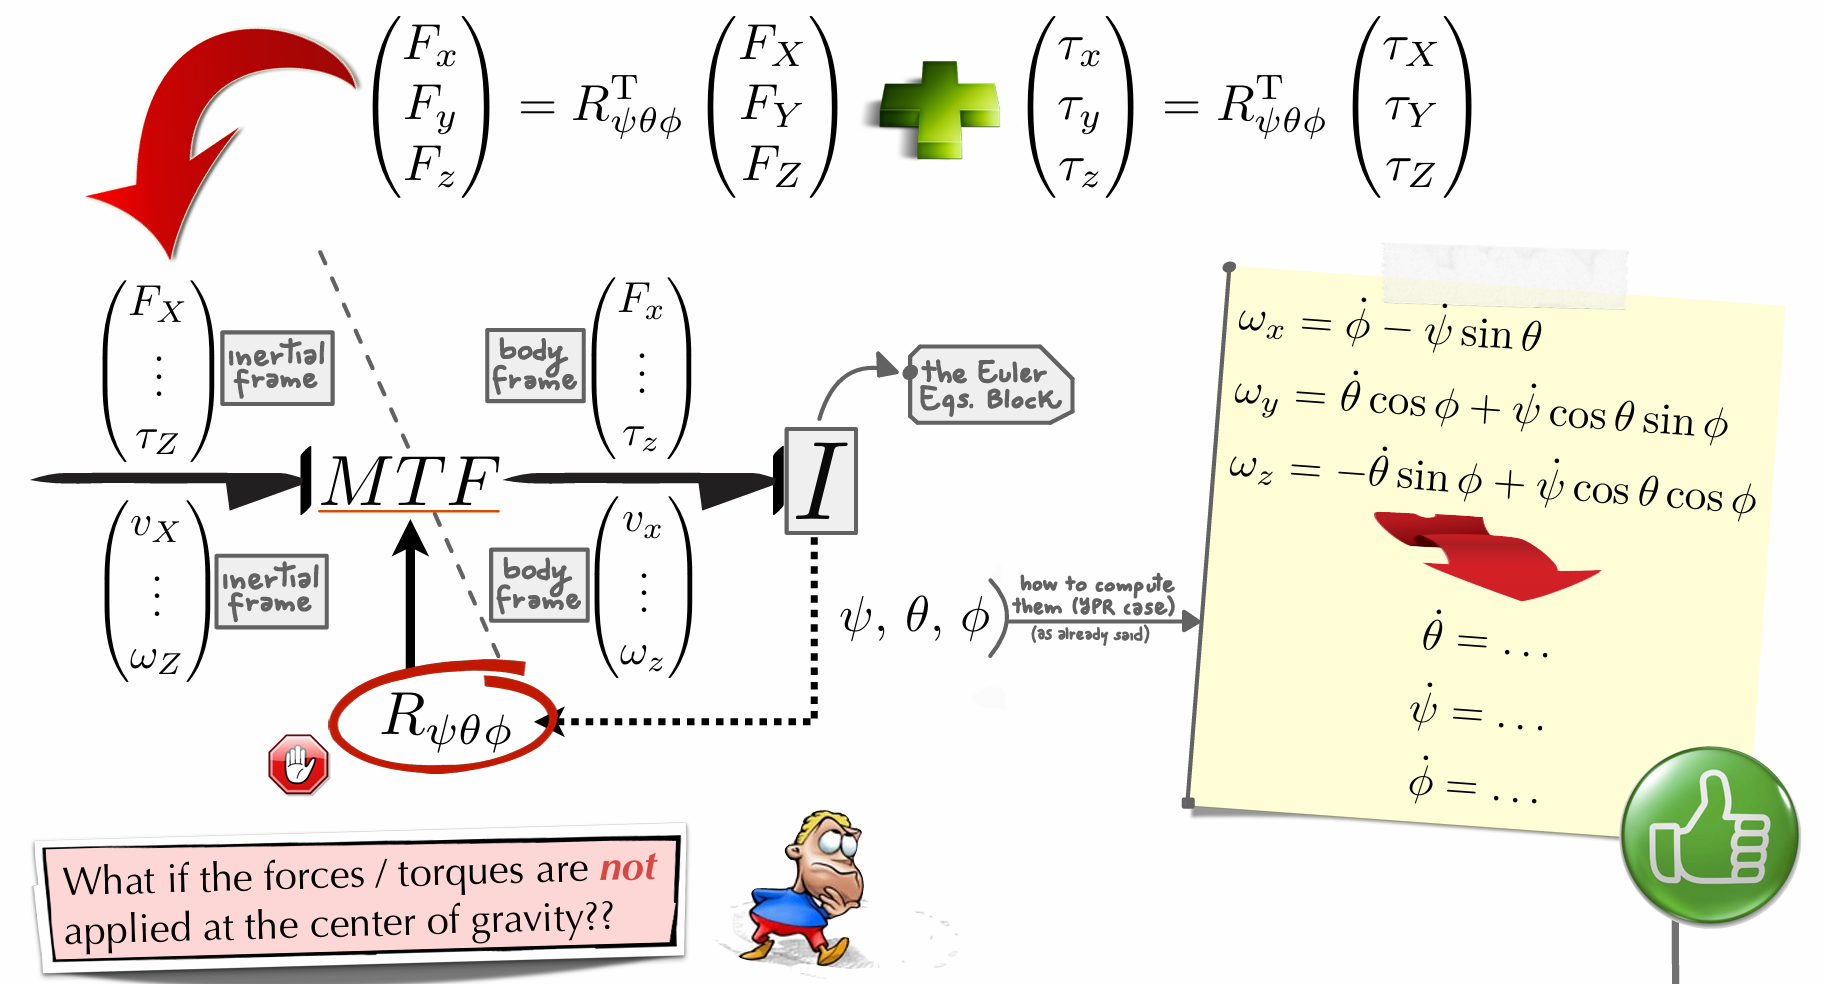
\includegraphics[width=0.8\textwidth]{figs/chapter6/6_5.png}
  \caption{The rotation matrix $\mathbf{R}$ acts as a modulated transformer (MTF) that converts body-frame velocities and forces to inertial-frame quantities, allowing us to connect the rigid body I-field to external forces and gravity defined in the inertial frame.}
\end{figure}


\paragraph{Forces not applied at the Centre of Gravity.}
Often, connecting forces are applied at a point $P$ offset from the CoG $G$ by a fixed vector $\mathbf{r}_{GP}$ in the body frame. The velocity of point $P$ is given by:
\begin{equation}
  \mathbf{v}_P = \mathbf{v}_G + \boldsymbol{\omega} \times \mathbf{r}_{GP}
\end{equation}
In matrix form, this kinematic relationship defines a \textbf{Body Frame Configuration Tensor} $\mathbf{T}(P)$:
\begin{equation}
  \begin{pmatrix}\mathbf{v}_P \\ \boldsymbol{\omega}\end{pmatrix} = \begin{pmatrix}\mathbf{I} & -\mathbf{r}_{GP}\times \\ \mathbf{0} & \mathbf{I}\end{pmatrix} \begin{pmatrix}\mathbf{v}_G \\ \boldsymbol{\omega}\end{pmatrix}
\end{equation}
By power conservation, the transposed tensor maps the forces applied at $P$ back to equivalent forces and torques at the CoG:
\begin{equation}
  \begin{pmatrix}\mathbf{F}_G \\ \boldsymbol{\tau}_G\end{pmatrix} = \begin{pmatrix}\mathbf{I} & \mathbf{0} \\ \mathbf{r}_{GP}\times & \mathbf{I}\end{pmatrix} \begin{pmatrix}\mathbf{F}_P \\ \boldsymbol{\tau}_P\end{pmatrix}
\end{equation}
This allows us to freely attach any number of forces or velocities applied at generic points using an MTF block.

\begin{figure}[H]
  \centering
  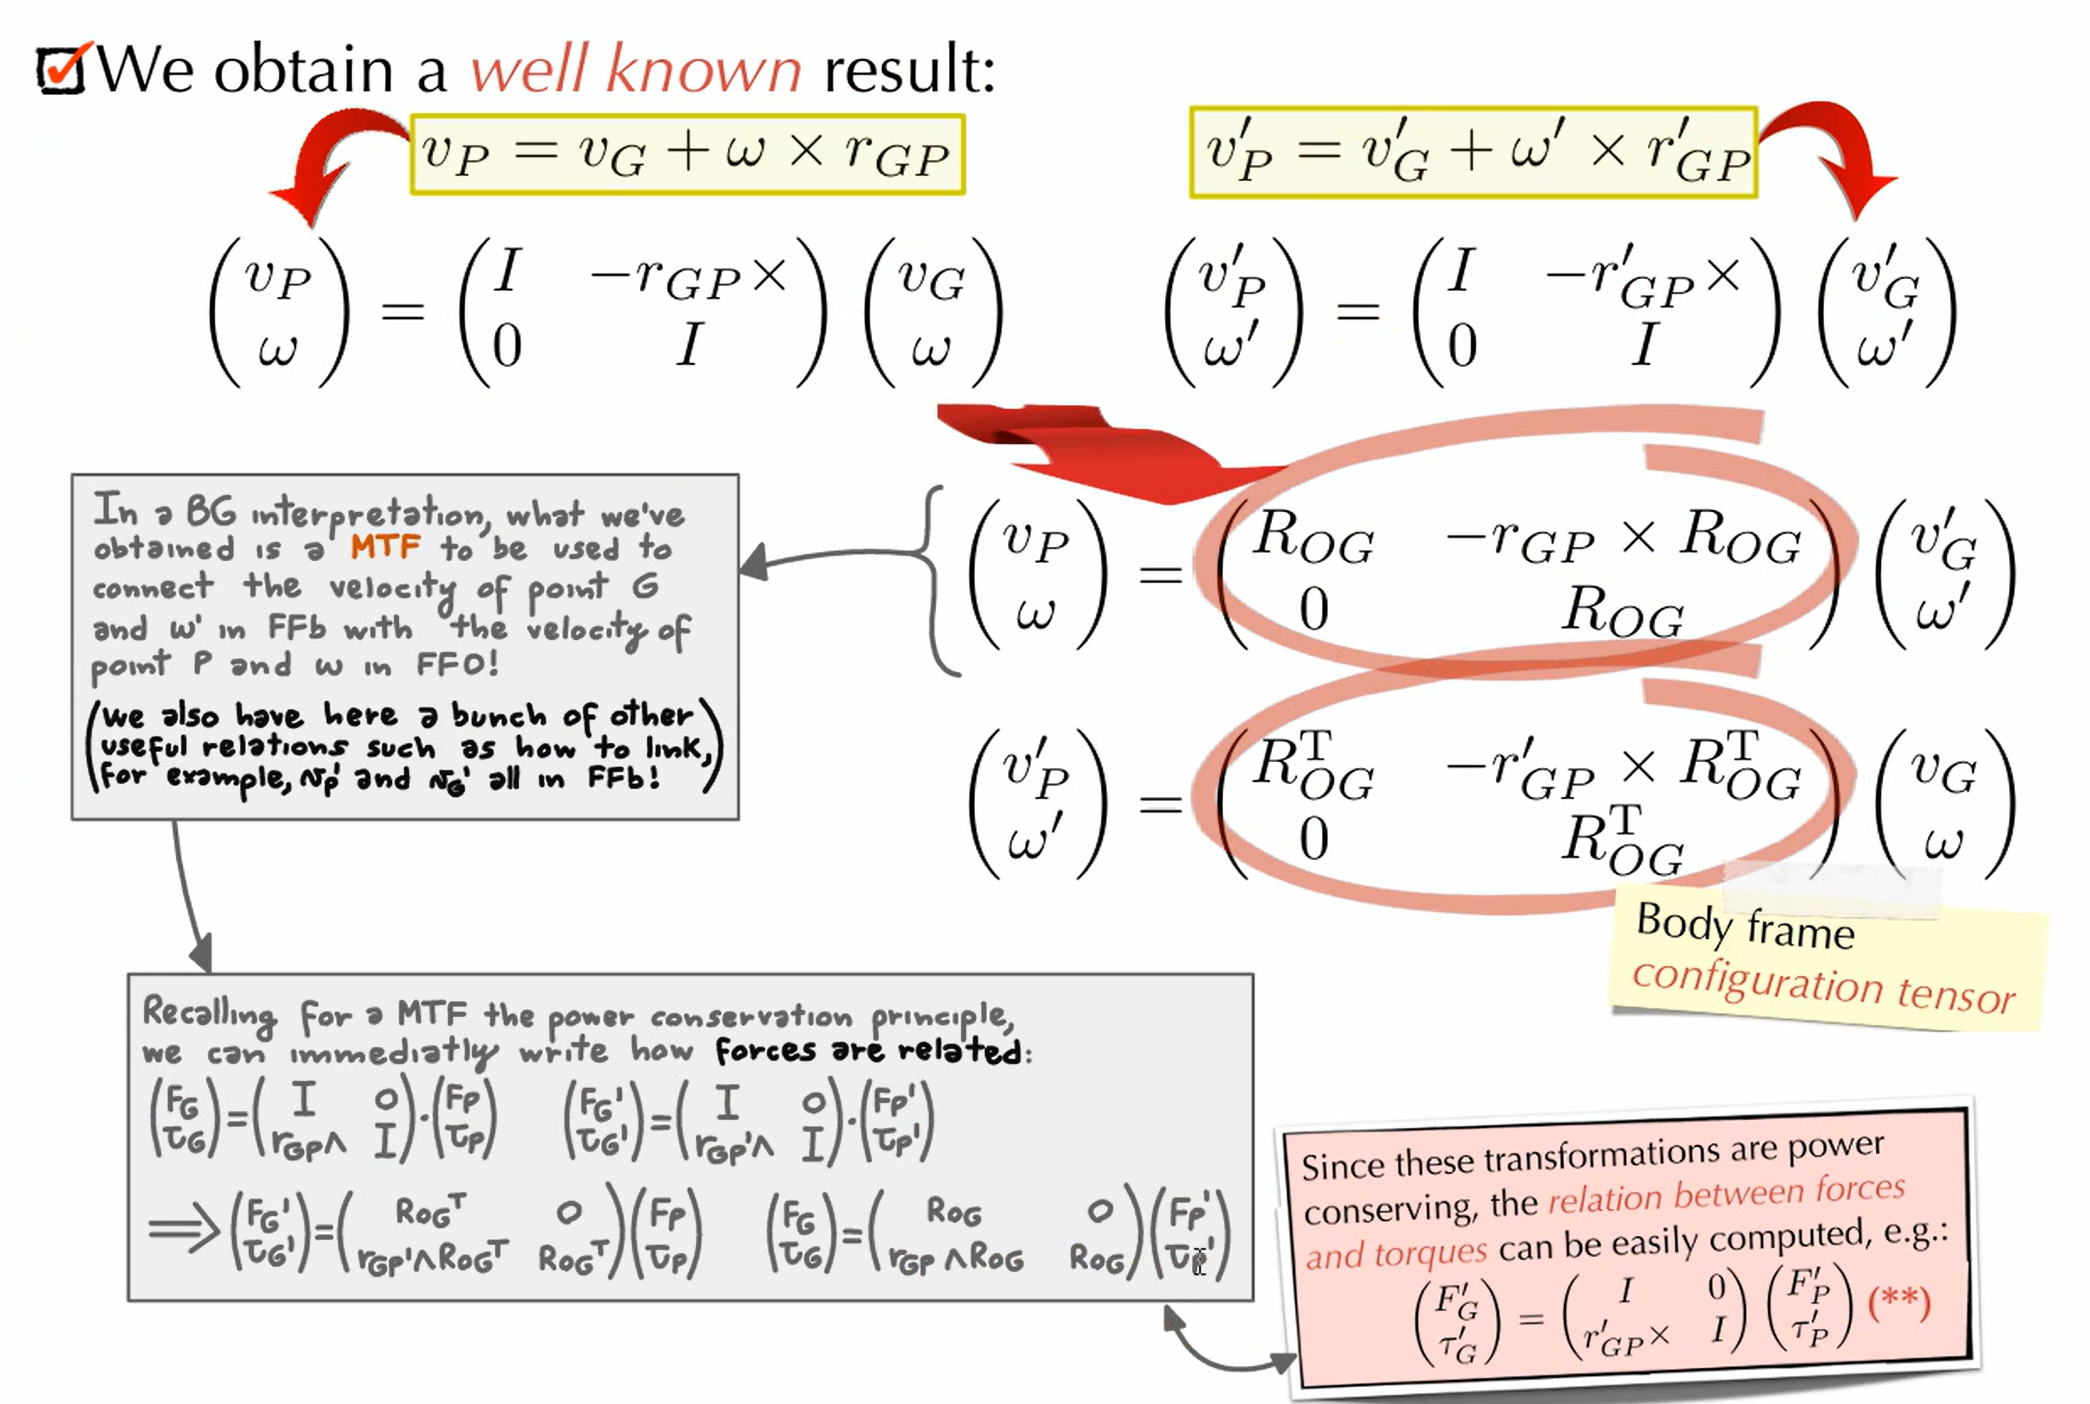
\includegraphics[width=0.8\textwidth]{figs/chapter6/6_6.png}
  \caption{Forces applied at a point $P$ offset from the CoG $G$ can be transformed to equivalent forces and torques at $G$ using a Body Frame Configuration Tensor $\mathbf{T}(P)$, which accounts for the lever arm effect of the offset.}
\end{figure}

We can write the whole rigid link bond graph in this manner: 

\begin{figure}[H]
  \centering
  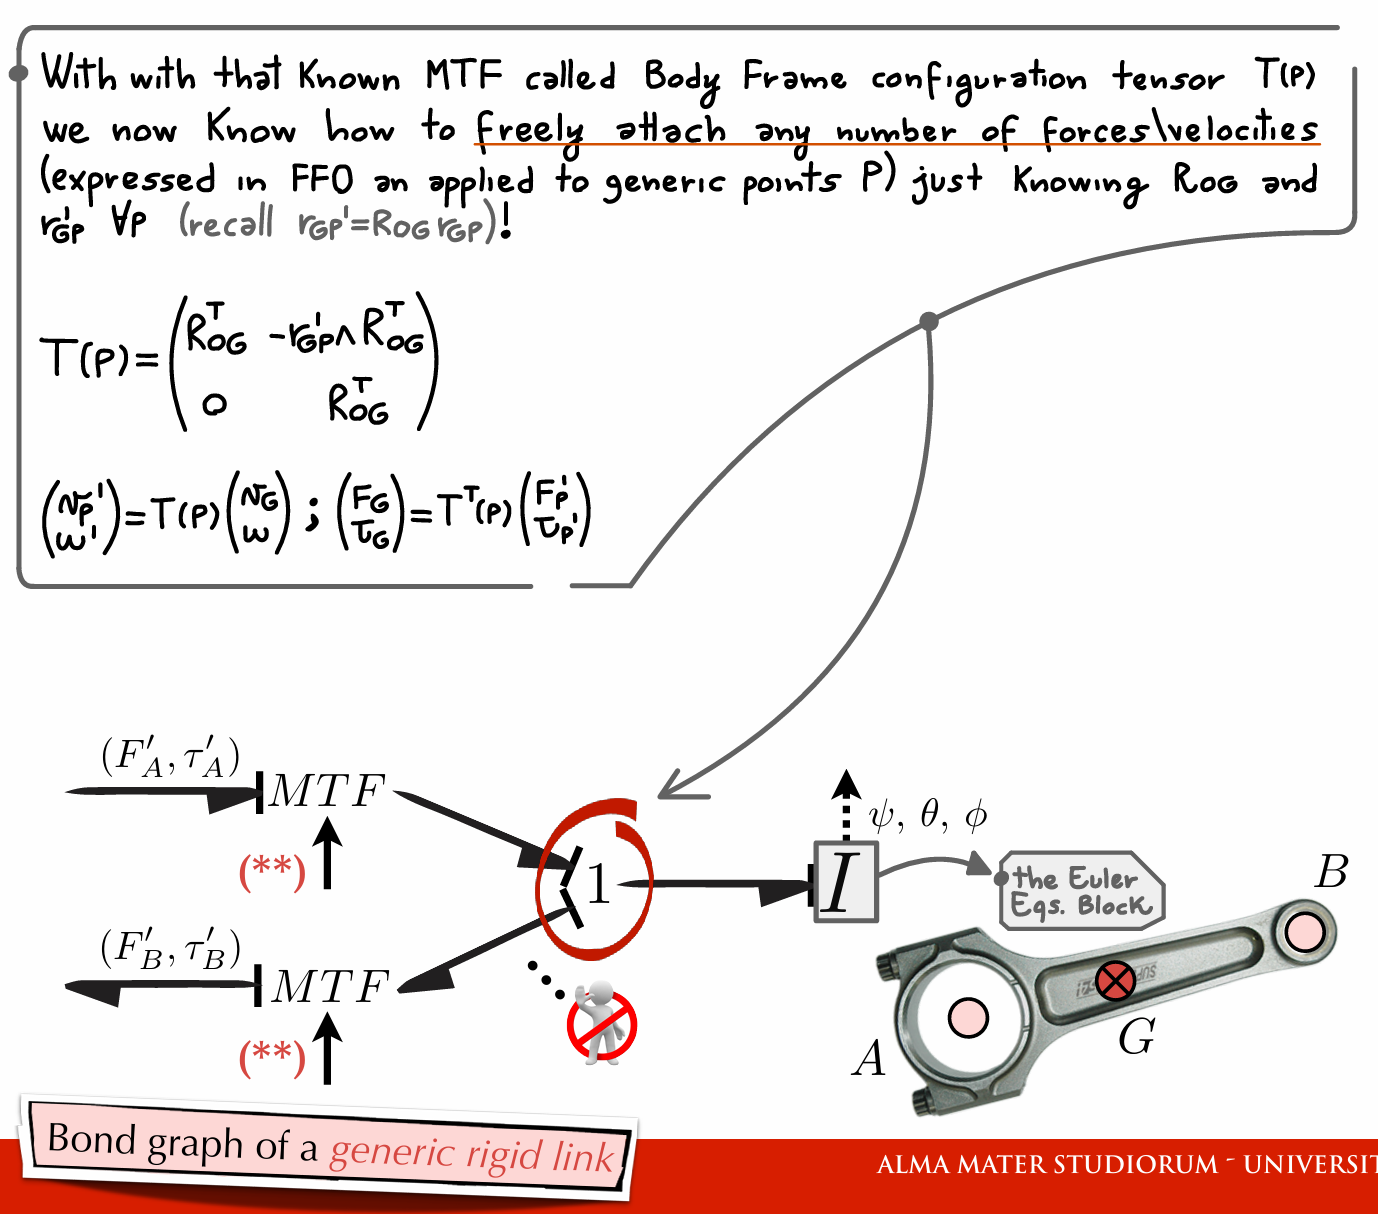
\includegraphics[width=0.8\textwidth]{figs/chapter6/6_7.png}
  \caption{The bond graph of a single rigid body in the inertial frame.}
\end{figure}

They are used to move from a point $A$ in the rigid body to a point $B$ in the same rigid body.

\section{Joints between rigid links}

A \textbf{joint} connects two rigid links by constraining their relative motion to a subspace. In the inertial frame:

\paragraph{Rotational (Revolute) joint.}
The relative linear velocity between the two attachment points is zero; the relative angular velocity $\omega_r = \omega_B - \omega_A$ is free (the joint can rotate). A torque $\tau_r$ acts along the joint axis. 
A revolute joint fully constrains linear velocities at the joint centre $P$, which is fixed with respect to both body frames. The bond graph imposes the velocity constraint via an MTF ($\mathbf{v}_P^A = \mathbf{R}_B^A \mathbf{v}_P^B$), and identifies the relative angular velocity:
\begin{equation}
  \mathbf{v}_A = \mathbf{v}_B \quad (\text{at the joint location}), \qquad
  \boldsymbol{\omega}_{AB}^A = \boldsymbol{\omega}_B^A - \boldsymbol{\omega}_A^A \text{ (free)}.
\end{equation}

\begin{figure}[H]
  \centering
  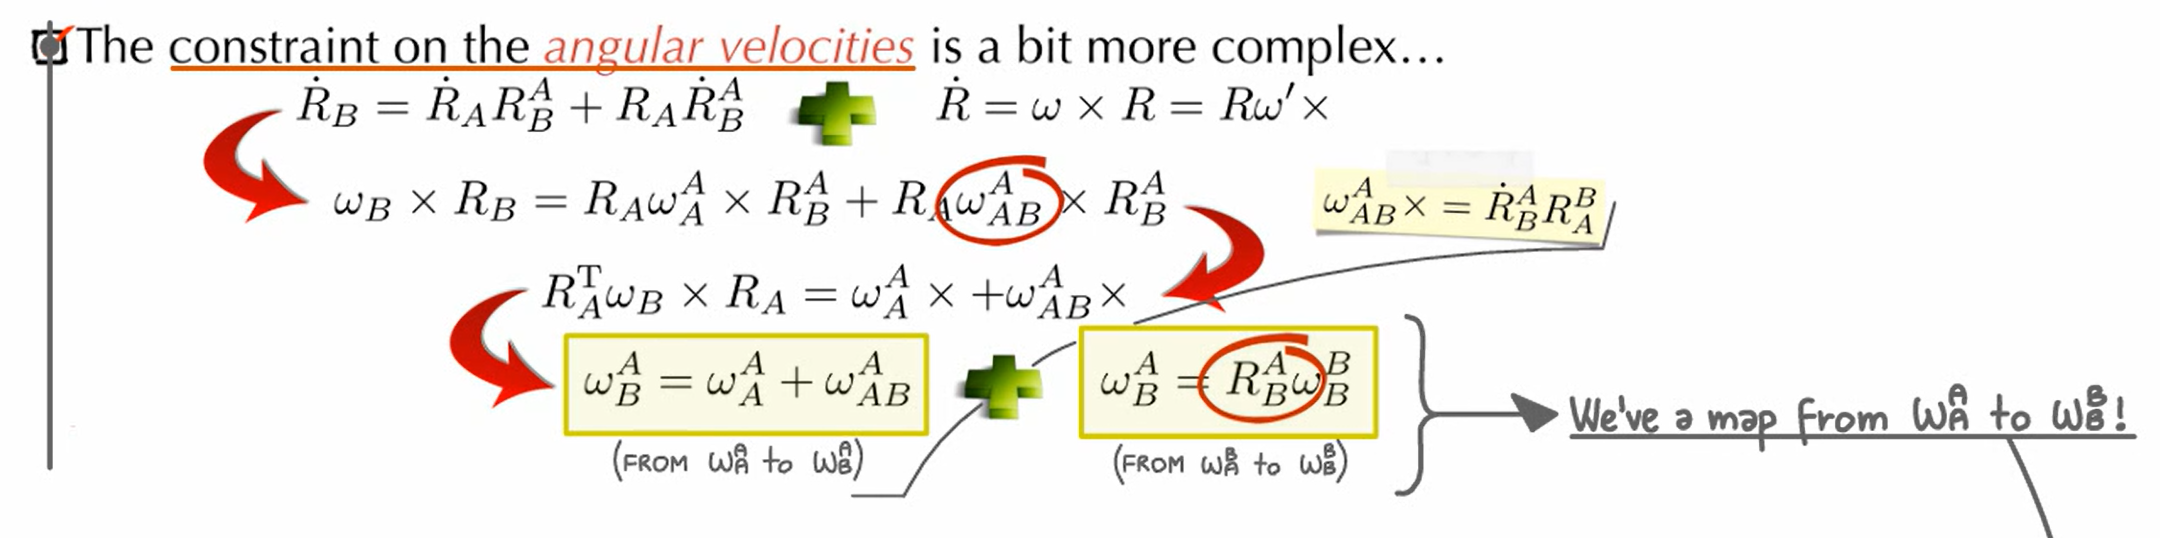
\includegraphics[width=0.8\textwidth]{figs/chapter6/6_8.png}
  \caption{Derivation of angular velocity formula}  
\end{figure}

Assuming the $z$-axis is oriented along the rotation axis, $\boldsymbol{\omega}_{AB}^A = (0, 0, \dot{\varphi})^T$.

Wrt inertial frame, the rotation matrix is: 
\begin{equation}
  \mathbf{R}_B = \mathbf{R}_A + \mathbf{R}_B^A
\end{equation}

The revolute joint can be modelled as followed, following the Denavit--Hartenberg convention for the joint axis and the relative angle 

\begin{figure} [H]
  \centering
  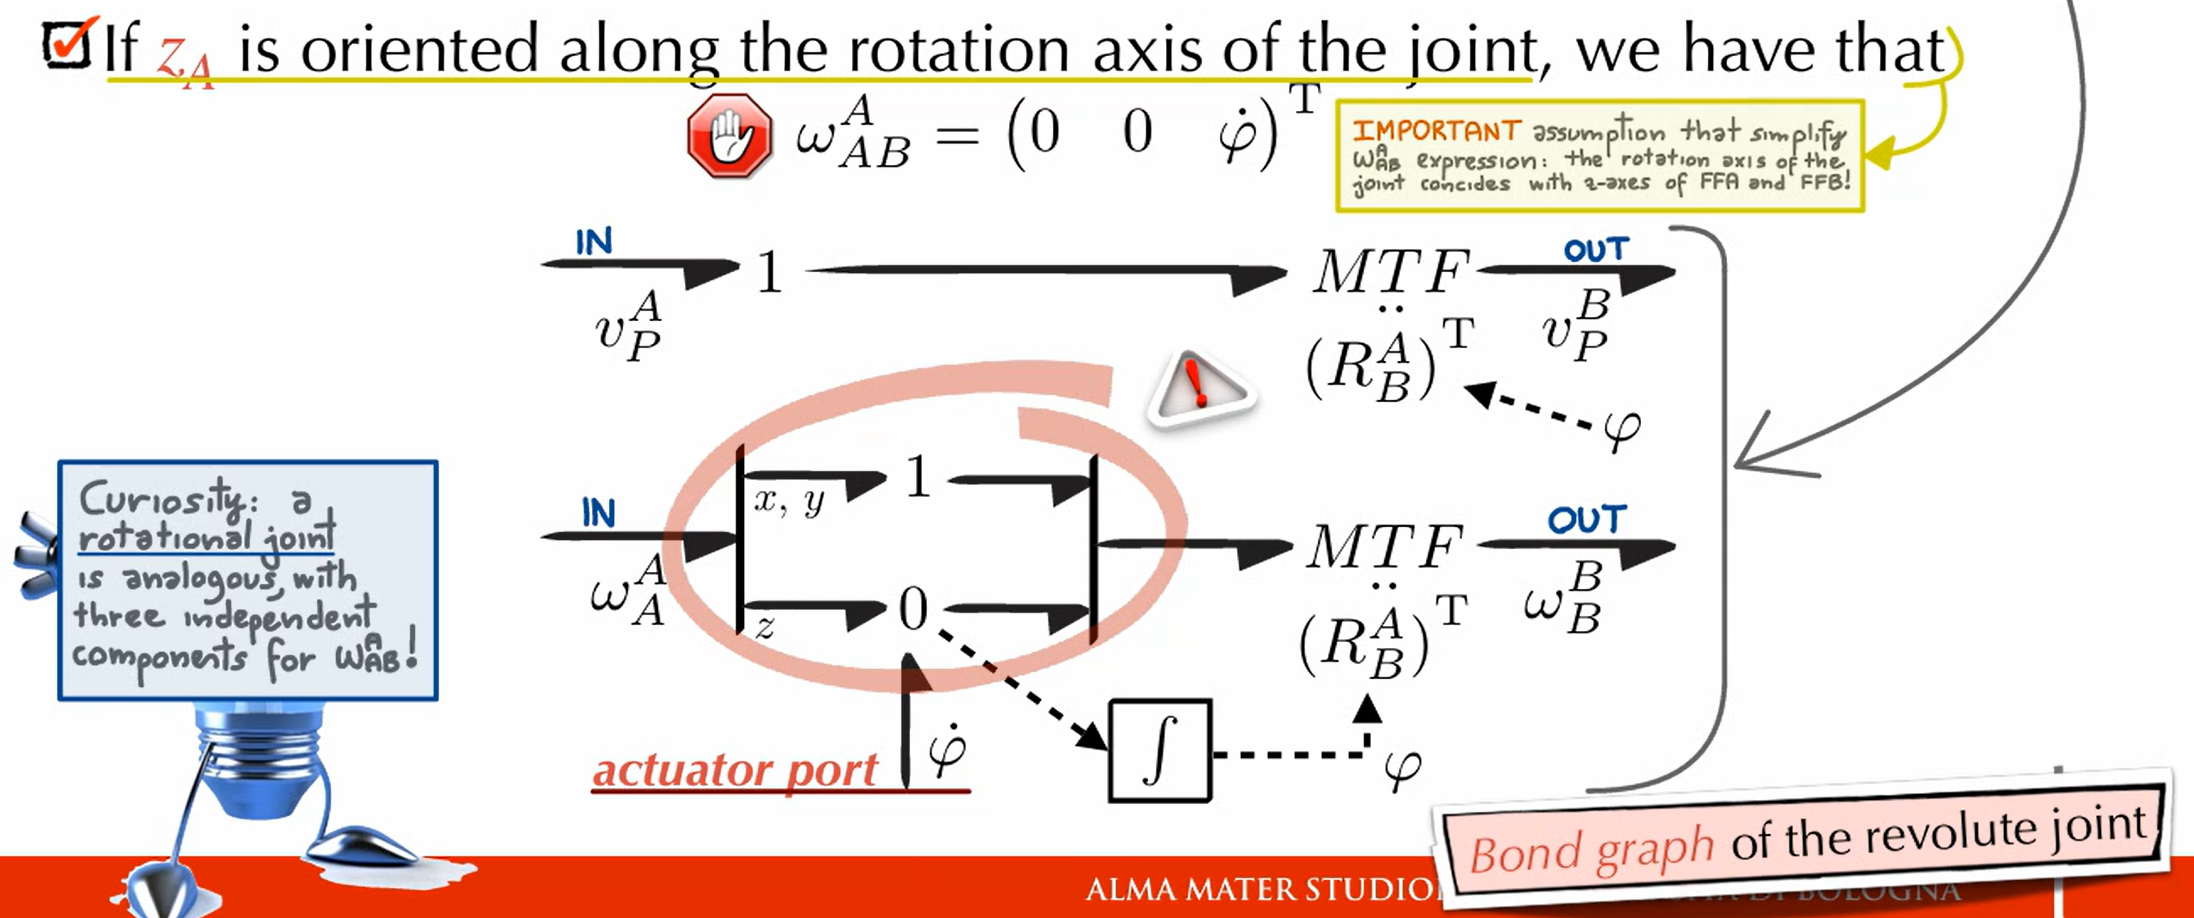
\includegraphics[width=0.8\textwidth]{figs/chapter6/6_9.png}
  \caption{Bond graph of a revolute joint between two rigid bodies, showing the velocity constraints and the free rotational degree of freedom.}
\end{figure}



\paragraph{Translational (Prismatic) joint.}
A prismatic joint fully constrains angular velocities among the bodies ($\boldsymbol{\omega}_A = \boldsymbol{\omega}_B$), meaning they always have the same relative orientation. The relative linear velocity is constrained to one direction $\hat{\mathbf{d}}(\theta)$ (which itself varies as the mechanism rotates). A force $F_r$ acts along this direction. Assuming the translation axis coincides with the $z$-axis of both frames, $\mathbf{v}_{AB}^A = (0, 0, \dot{s})^T$. The constraint and the direction transformation involve MTF elements with time-varying moduli that depend on the current configuration angle $\theta$.

\begin{figure} [H]
  \centering
  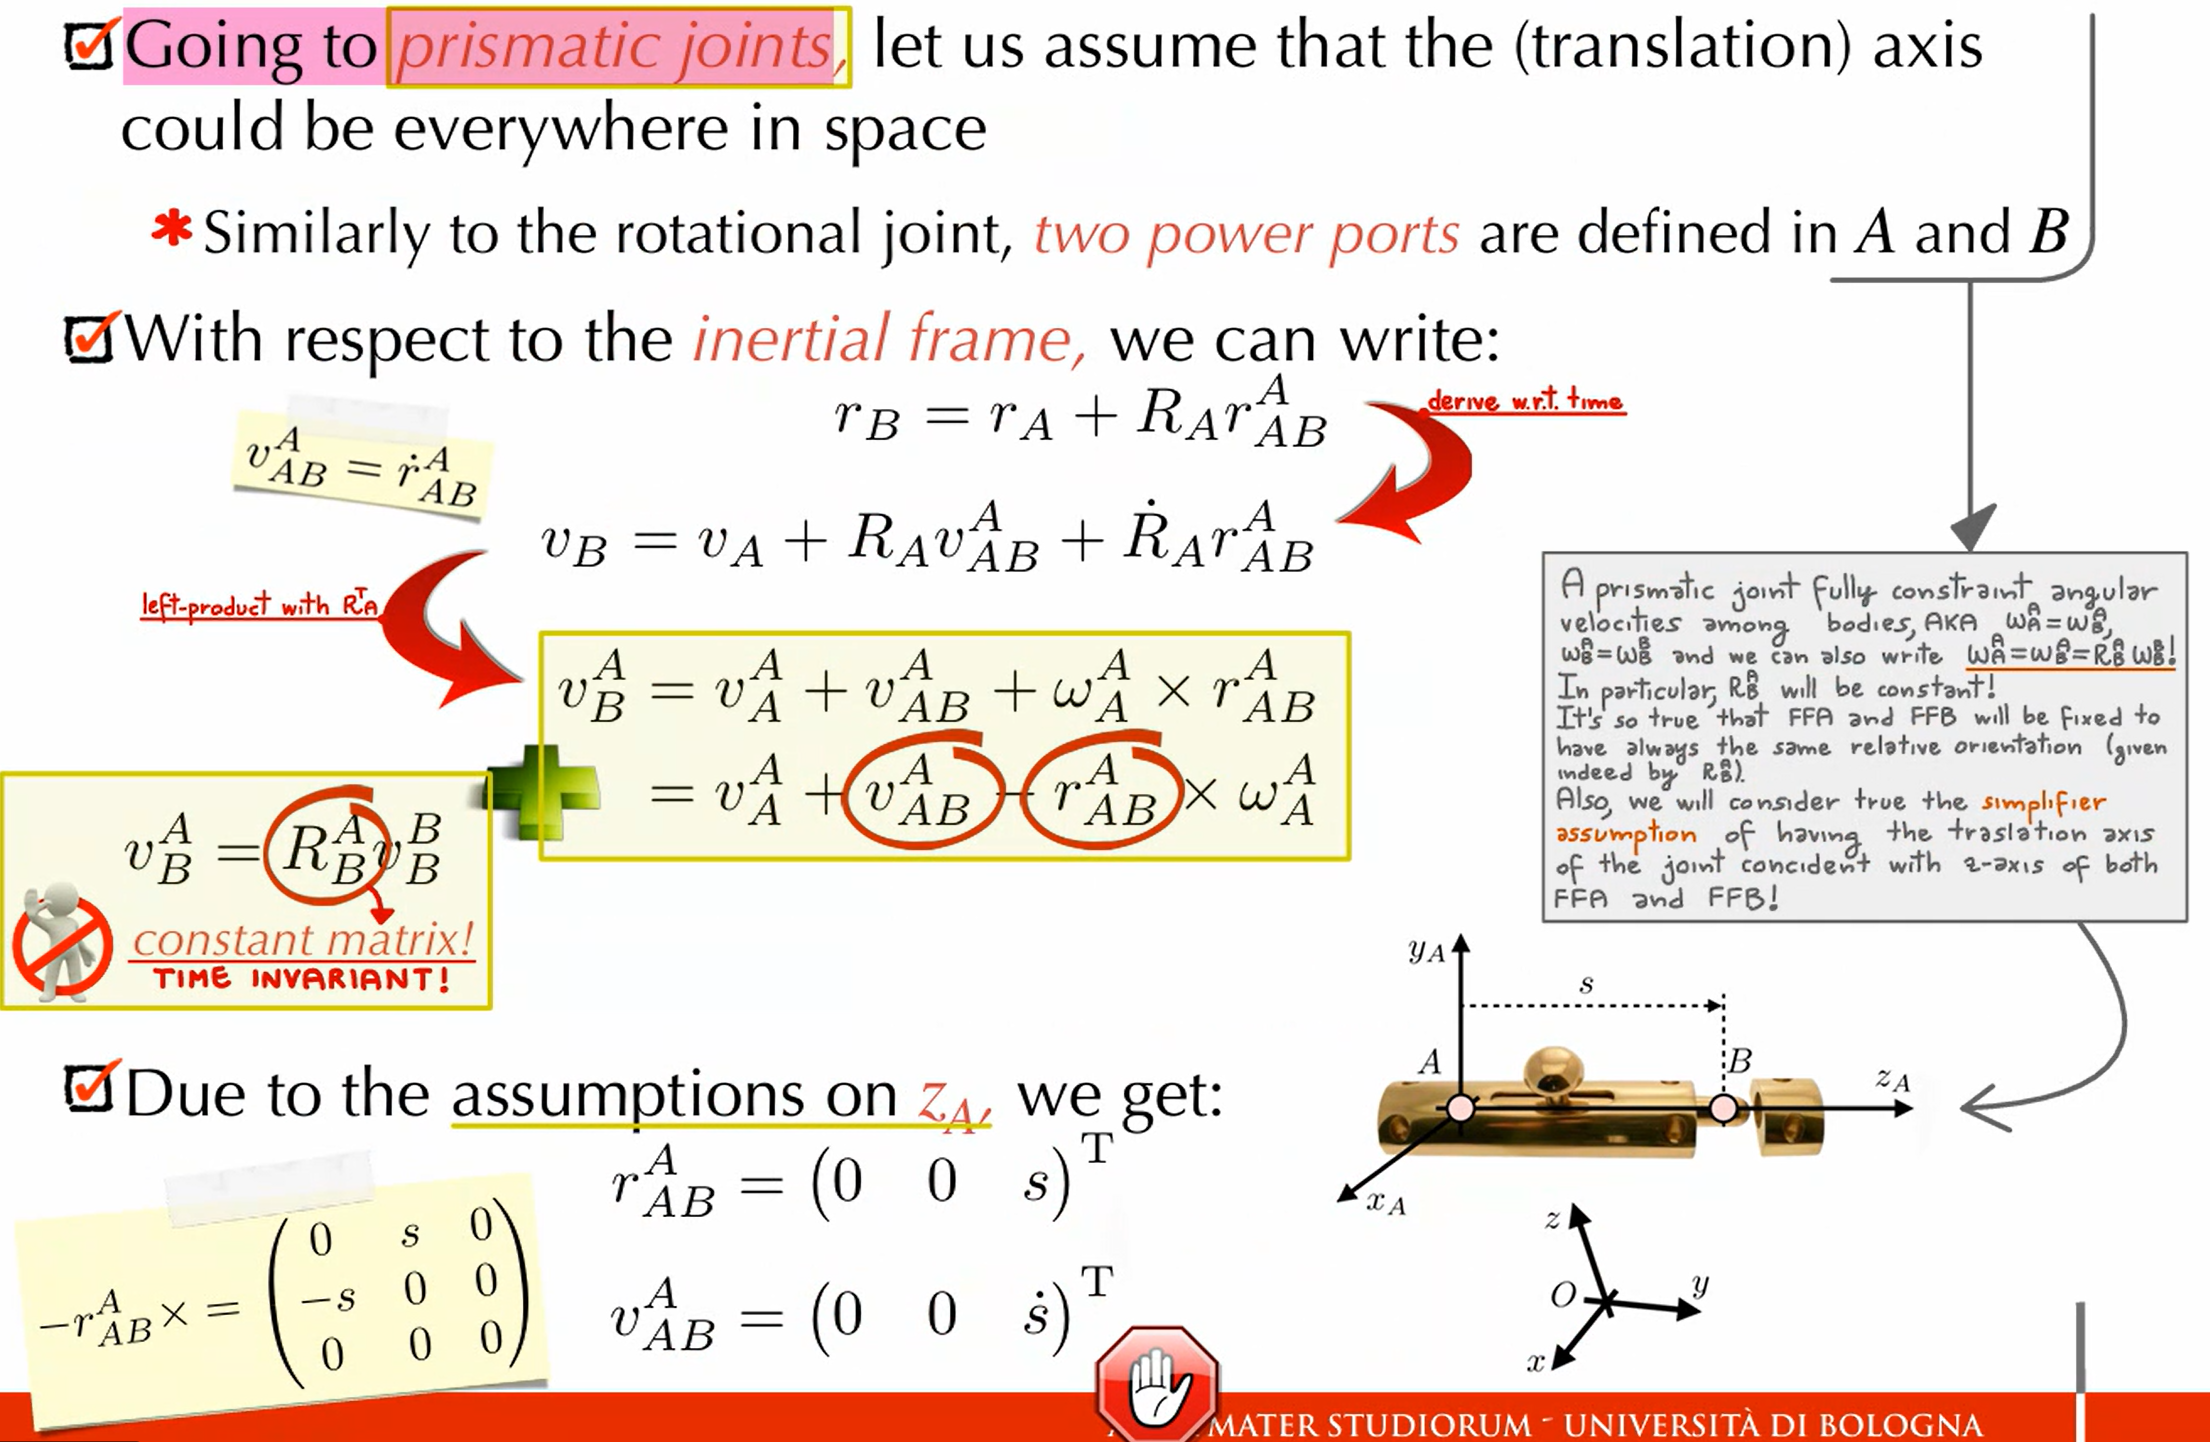
\includegraphics[width=0.8\textwidth]{figs/chapter6/6_10.png}
  \caption{Derivation of equations for a prismatic joint, plus assumption of Denavit--Hartenberg convention for the joint axis.}
\end{figure}


The key practical point is: in the inertial-frame formulation, joint directions $\hat{\mathbf{d}}(\theta)$ are time-varying, making the MTF moduli time-varying. This is why the \textbf{body-frame formulation} is typically preferred for multi-body dynamics — joint directions remain constant in the body frame.

\begin{figure} [H]
  \centering
  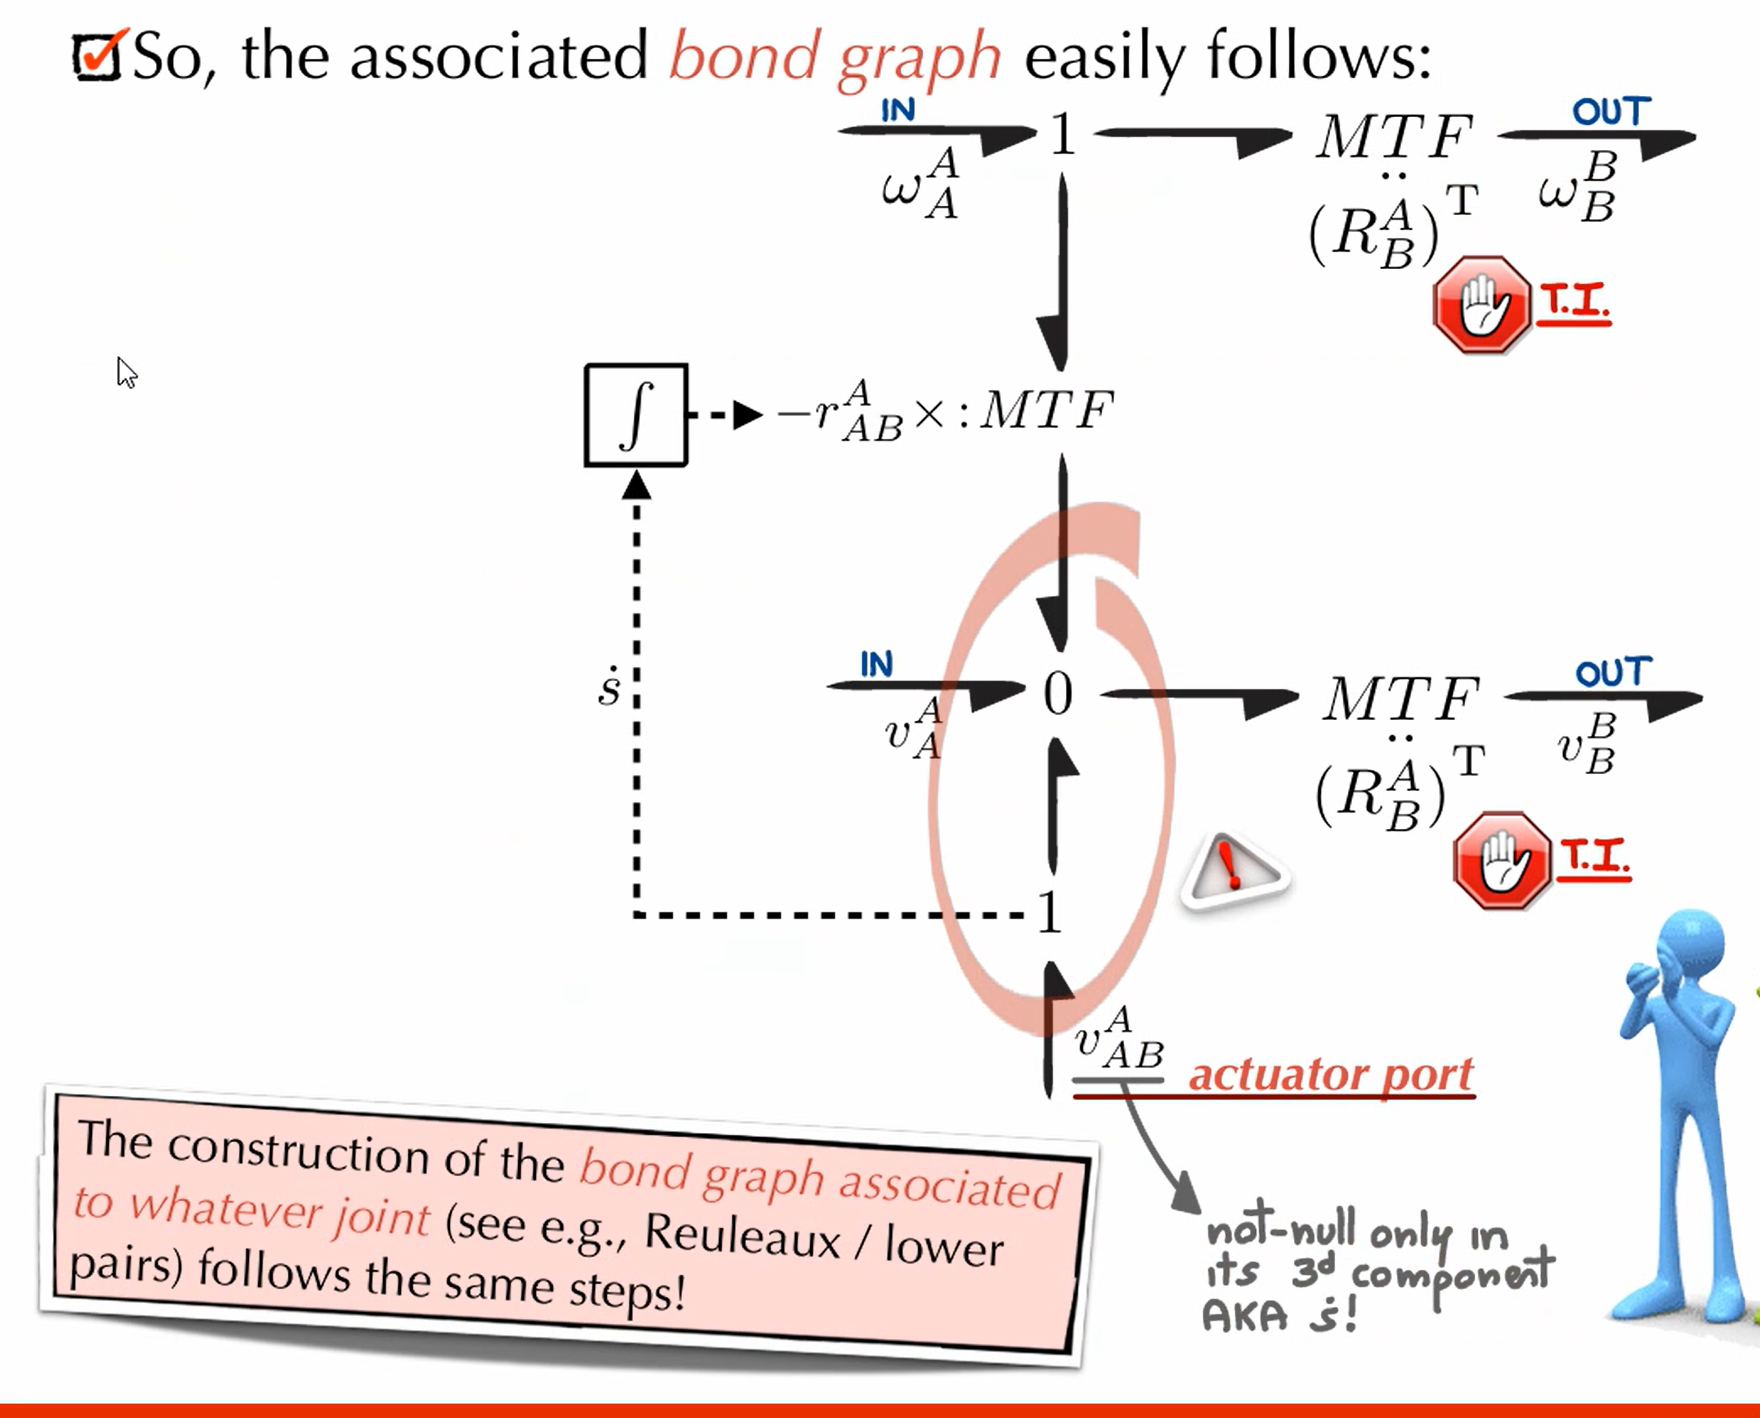
\includegraphics[width=0.8\textwidth]{figs/chapter6/6_11.png}
  \caption{Bond graph of a prismatic joint between two rigid bodies, showing the angular velocity constraints and the linear velocity constraint along the prismatic axis.}
\end{figure}







\section{Kinematic nonlinearities in the dynamics}

Main drawback is that the final equations are nonlinear and with (integrable) constraint. Up to now we just used the kinematic constraints to write the bond graph, we haven't yet introduced the dynamics of the system. For simpler systems using the proposed method is too complex.

We must find a convenient way to describe the system without the rigid body dynamics. We'll use a \textbf{standard model}. 


For any problem in mechanics involving particles, rigid bodies and elastic elements, the mathematical model consists of a set of first order ODEs in terms of variables with some physical insight.

Equations are \textbf{coupled} and \textbf{explicit}. 

\begin{align}
  f_C = \Phi_C^{-1} (q_C) \\
  v_I = \Phi_I^{-1} (p_I) \\
  \dot{q}_C = T_{CI} (q_C) v_I \\
  \dot{p}_I = - T_{CI}^T (q_C) f_C
\end{align}


The most difficult aspect is the nonlinear coupling of C- and I- fields introduced by the geometry of large-scale motions, i.e. $T_{CI}(q_C)$ by that is associated with multiport displacement-modulated transformers

Forces and velocities $(f_C, v_I)$ can be eliminated which gives:

\begin{equation*}
  \dot{q}_C = T_{CI}(q_C) \Phi_I^{-1} (p_I), \qquad
  \dot{p}_I = - T_{CI}^T (q_C) \Phi_C (q_C)
\end{equation*}

\begin{figure} [H]
  \centering
  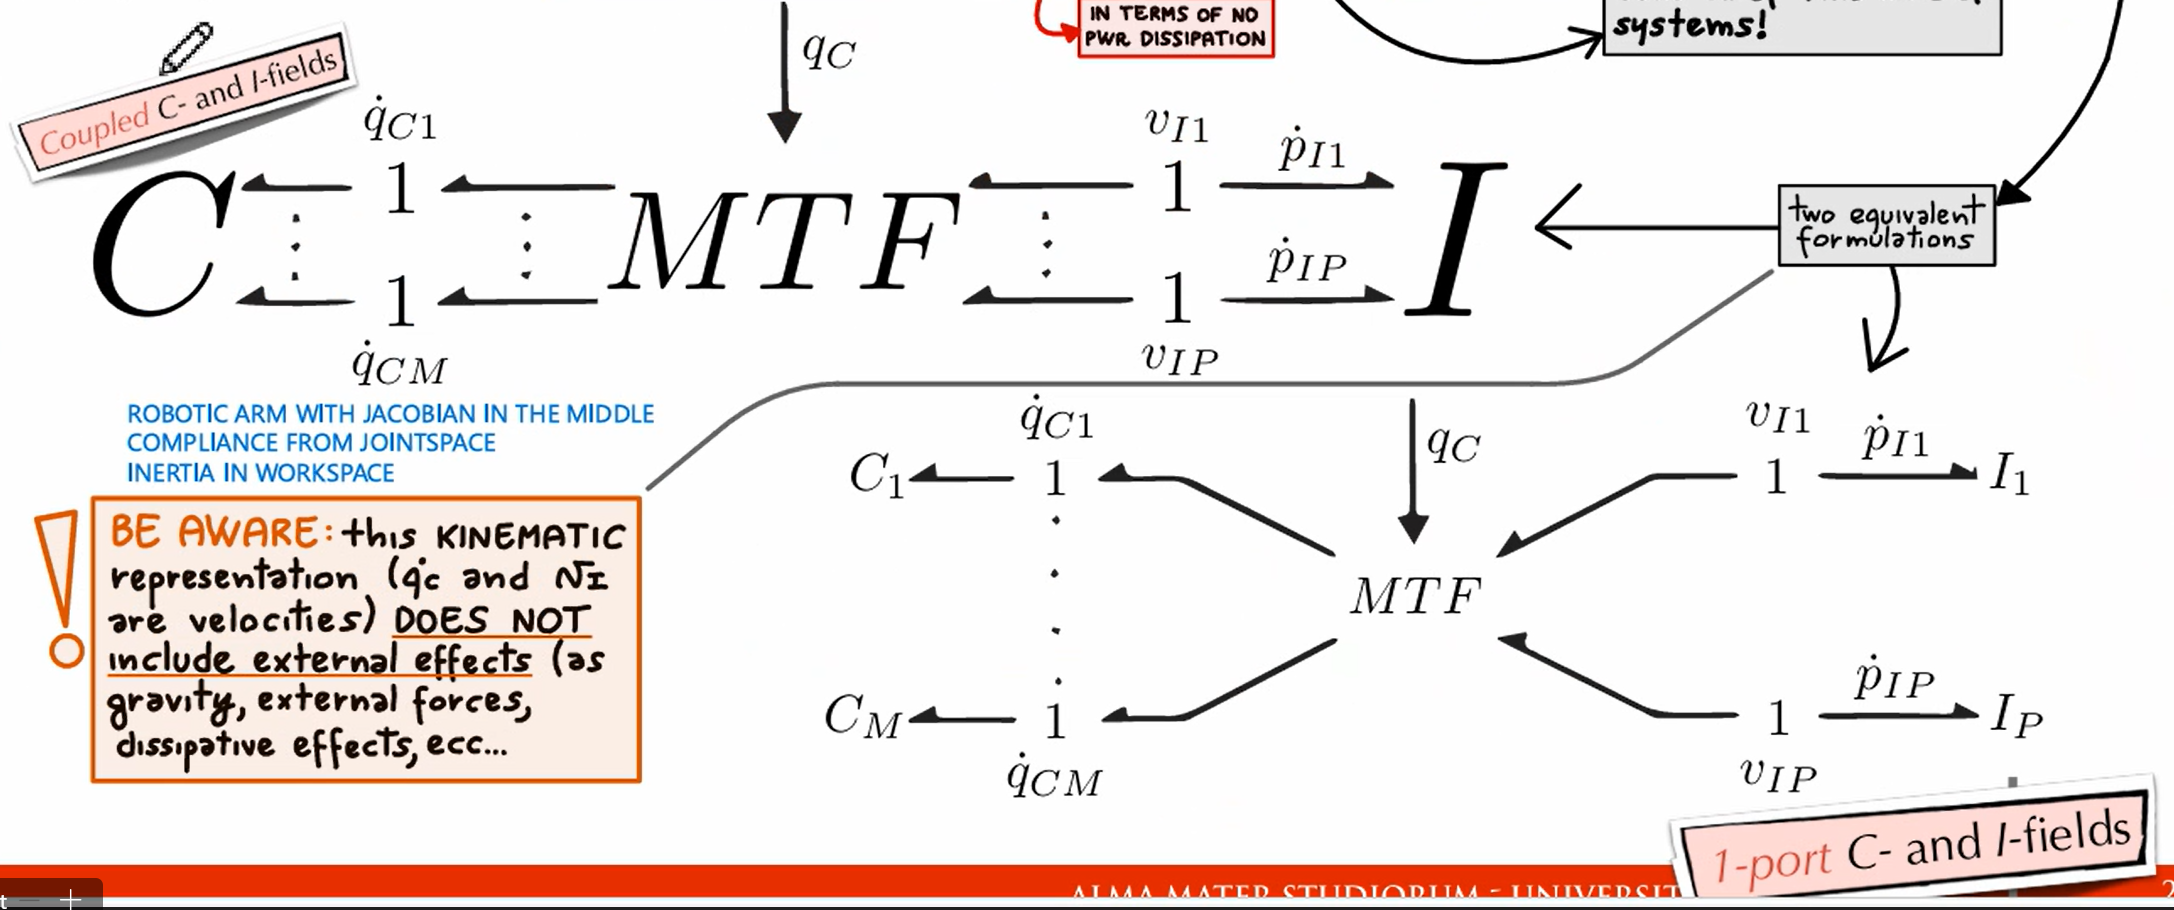
\includegraphics[width=0.8\textwidth]{figs/chapter6/6_12.png}
  \caption{Basic nonlinear conservative system}
\end{figure}

Here is an example with the spring-pendulum. Notice that it's possible to add external forces. 

\begin{figure} [H]
  \centering
  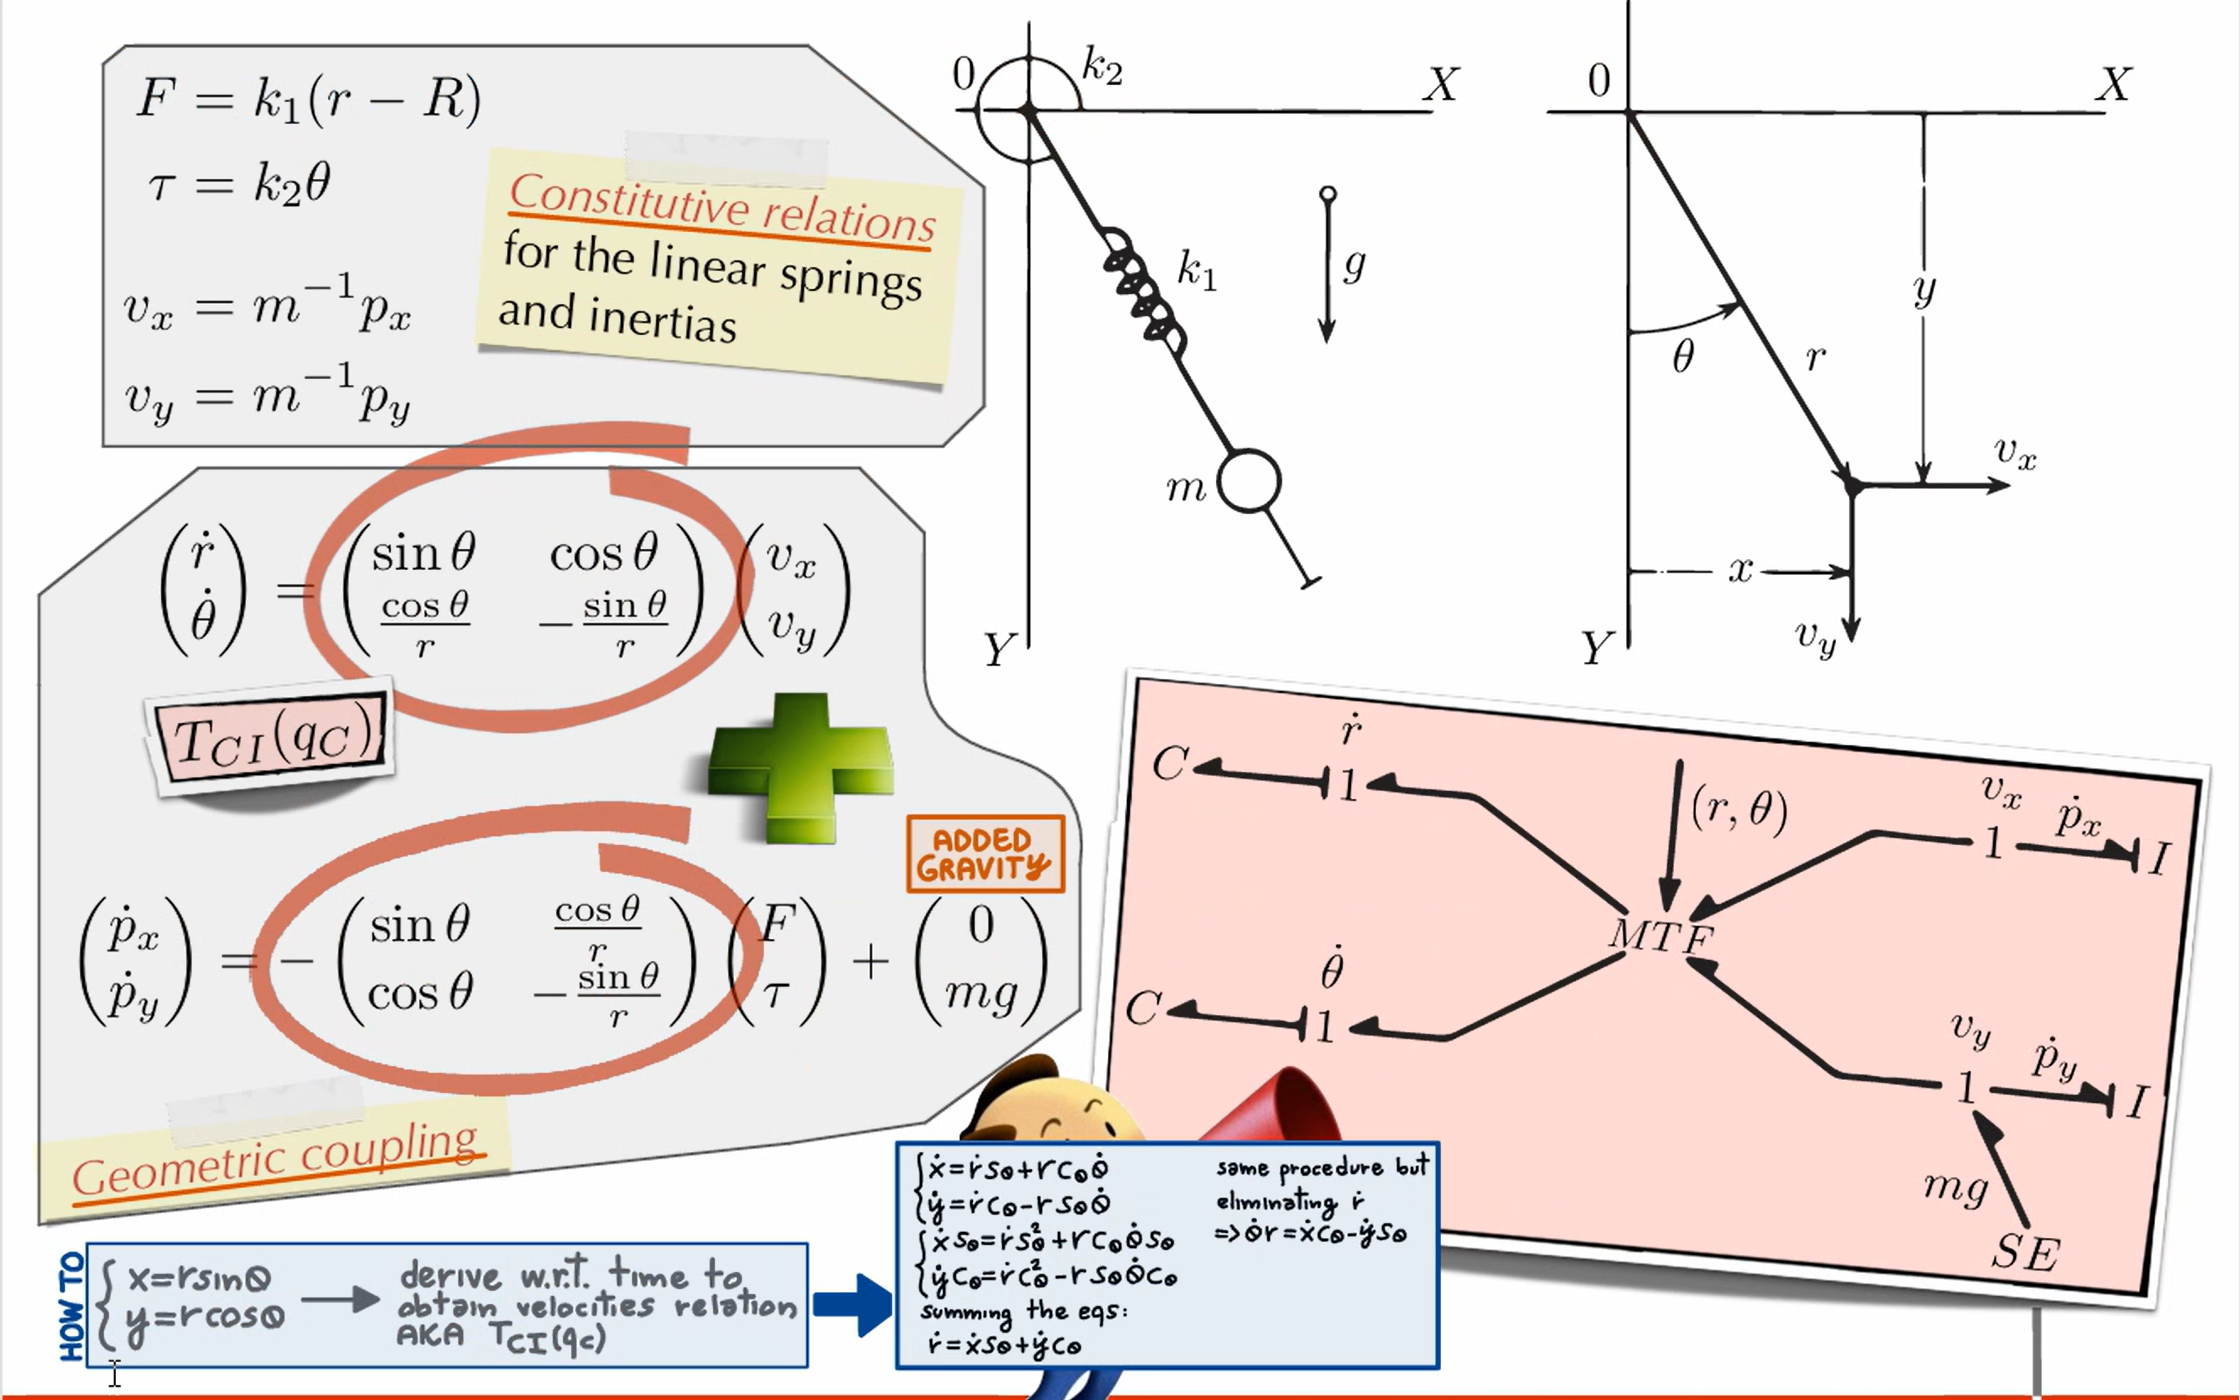
\includegraphics[width=0.8\textwidth]{figs/chapter6/6_13.png}
  \caption{Spring pendulum example}
\end{figure}

This is a conservative system, so there are no damping terms. 


\section{The K.A.M. (Kinematic Analysis Method)}

Before addressing closed loops and derivative causality, it is useful to formalize how to build a mechanism's bond graph starting purely from kinematics.
\begin{enumerate}[leftmargin=2em,itemsep=2pt]
  \item \textbf{Identify key variables}: Determine the vector of generalized coordinates $\mathbf{q}_k$, the C-field displacements $\mathbf{q}_C$, and the I-field velocities $\mathbf{v}_I$. Note that this method works with velocities (flows).
  \begin{enumerate}
    \item If the vector containing the time derivatives of the generalised coordinates  $q_k$ represents a necessary and sufficient set of velocities to fix all the motions at any instant, then the system is holonomic
  \end{enumerate}
  \item \textbf{C-field constraints}: Relate $\mathbf{q}_C$ to $\mathbf{q}_k$ and differentiate to get $\dot{\mathbf{q}}_C = \mathbf{T}_{Ck}(\mathbf{q}_k)\dot{\mathbf{q}}_k$. Write this into the bond graph using MTFs and 0-junctions.
  \item \textbf{I-field constraints}: Obtain the velocity transformation $\mathbf{v}_I = \mathbf{T}_{Ik}(\mathbf{q}_k)\dot{\mathbf{q}}_k$ and append to the graph via MTFs.
  \item \textbf{Attach elements}: Append C- and I-fields to their respective junctions. Add dissipation, gravity (as SE), and simplify the MTFs where possible.
\end{enumerate}



This kinematic description uses a junction structure that links flows (assumed to depend on C-energy variables) to couple C-fields and I-fields. However, this procedure often leads to bond graphs with algebraic loops or derivative causality when bodies are rigidly constrained.


\paragraph{}
The procedure is often successful at deriving a bond graph what will yield state equations easily but it can lead to algebraic loops or with derivative causality. 
A serious problem occurs when two rigid bodies are constrained in a non-flexible way. 


\section{Introduction to DAEs vs ODEs}
In standard Ordinary Differential Equations (ODEs), the system states are defined by explicit derivatives (e.g., accelerations), which a numerical solver integrates to find velocities and positions. A Differential-Algebraic Equation (DAE) introduces algebraic constraints alongside differential equations. The solver must satisfy both the integration steps and the strict algebraic rules simultaneously.

\section{Major Problems with DAEs}
\subsection{The Index Problem (Hidden Derivatives)}
Standard solvers integrate derivatives, meaning they cannot directly handle pure algebraic equations (which lack time derivatives). To solve the system, the algebraic constraint must be differentiated with respect to time until the required derivatives appear. The number of differentiations required is called the \textbf{Differential Index}. Most rigid multibody systems are Index-3 DAEs, which are mathematically heavy and unstable to solve directly.

\subsection{Constraint Drift}
When an algebraic constraint (e.g., position) is differentiated into a velocity or acceleration constraint, the solver ensures only the differentiated constraint is met. Due to tiny numerical truncation errors during integration, the uncorrected position variables will slowly diverge from the original algebraic constraint, causing the physical system to literally drift apart.

\section{Classic Example: The Rigid Pendulum}
Consider a pendulum with mass $m$ attached to a rigid, massless rod of length $L$. Modeled in Cartesian coordinates $(x, y)$, this forms a DAE.

\textbf{1. Differential Equations (Newton's Laws):}
Using $\lambda$ for the unknown tension magnitude:
\begin{align}
m\ddot{x} &= -x\lambda \
m\ddot{y} &= -y\lambda - mg
\end{align}

\textbf{2. Algebraic Equation (The Constraint):}
The rigid rod forces the mass to remain on a circle of radius $L$:
\begin{equation}
x^2 + y^2 - L^2 = 0
\end{equation}

\textbf{Solving and Drift:}
Since $\lambda$ does not appear in the constraint, we must differentiate the constraint twice (Index-3) to find the accelerations:
\begin{equation}
2x\ddot{x} + 2\dot{x}^2 + 2y\ddot{y} + 2\dot{y}^2 = 0
\end{equation}
Substituting Newton's laws into this allows us to solve for $\lambda$. However, because the solver is now strictly enforcing the \textit{acceleration} constraint, microscopic integration errors accumulate over time. The solver forgets the original $x^2 + y^2 = L^2$ rule, leading to constraint drift where the rigid rod slowly stretches and breaks apart in the simulation.


\textbf{Constraints} might be enforced by a joint between the bodies. The degrees of freedom are reduced
by the constraints and this always lead to derivative causality. 


\section{Multi-body problem and constraints}

When two rigid bodies are rigidly connected (e.g.\ a robotic link assembly), the degrees of freedom are reduced by the constraints. A rigid body requires six I-elements, but if rigidly connected, their velocities cannot all be independent. The naive bond graph has \emph{velocity constraints} that force some storage elements into derivative causality, signalling an inconsistency in the model. This is the classic \textbf{Multi-Body Problem}.

\subsection{The "Gaps Method" and Lagrange Multipliers (DAE formulation)}
If we treat the constraints mathematically, we define "gap variables" $\boldsymbol{\delta}$ (e.g., horizontal and vertical distances between two theoretically pinned joints) which must vanish ($\boldsymbol{\delta} = \mathbf{0}$). The forces required to enforce these gaps are \textbf{Lagrange Multipliers} ($\boldsymbol{\lambda}$). 
The system is written in a \emph{descriptor form} (a Differential-Algebraic Equation, DAE system), where $E\dot{\mathbf{x}} = A\mathbf{x} + B\mathbf{u}$ and matrix $E$ is singular. The Jacobian of the constraints $\boldsymbol{\Delta} = \partial \boldsymbol{\delta} / \partial \mathbf{q}_k$ relates the velocities ($\dot{\boldsymbol{\delta}} = \boldsymbol{\Delta}\dot{\mathbf{q}}_k$) and the constraint forces ($\mathbf{F}_e = \boldsymbol{\Delta}^T\boldsymbol{\lambda}$). In the bond graph, these appear as external forces opposing the natural motion to keep $\dot{\boldsymbol{\delta}} = 0$.

\subsection{Handling Derivative Causality Physically and Algebraically}
To resolve the derivative causality natively in the simulation, two distinct tricks are widely used:

\paragraph{Method 1: The "Parasitic Spring" (Breaking the Constraint).}
This is a highly practical engineering approach. Physically, two perfectly rigid bodies connected by a rigid joint represent an over-constrained idealisation. In reality, nothing is perfectly rigid; everything flexes. 
The resolution is to introduce a small \textbf{compliance} at the connection. Rather than a rigid bond forcing equal velocities via a strict 1-junction, the joint is modelled as a stiff spring (C-element with large $k$) and a small damper (R-element) between them.
This:
\begin{enumerate}[leftmargin=2em,itemsep=2pt]
  \item Breaks the strict kinematic constraint, restoring all C- and I-elements to integral causality because the masses can now vibrate at slightly different speeds.
  \item Introduces a fast time scale (stiff ODE) associated with the high-frequency compliance vibration. Stiff ODE solvers are required.
  \item Is physically correct — real connections always have some finite stiffness.
\end{enumerate}

\begin{figure} [H]
  \centering
  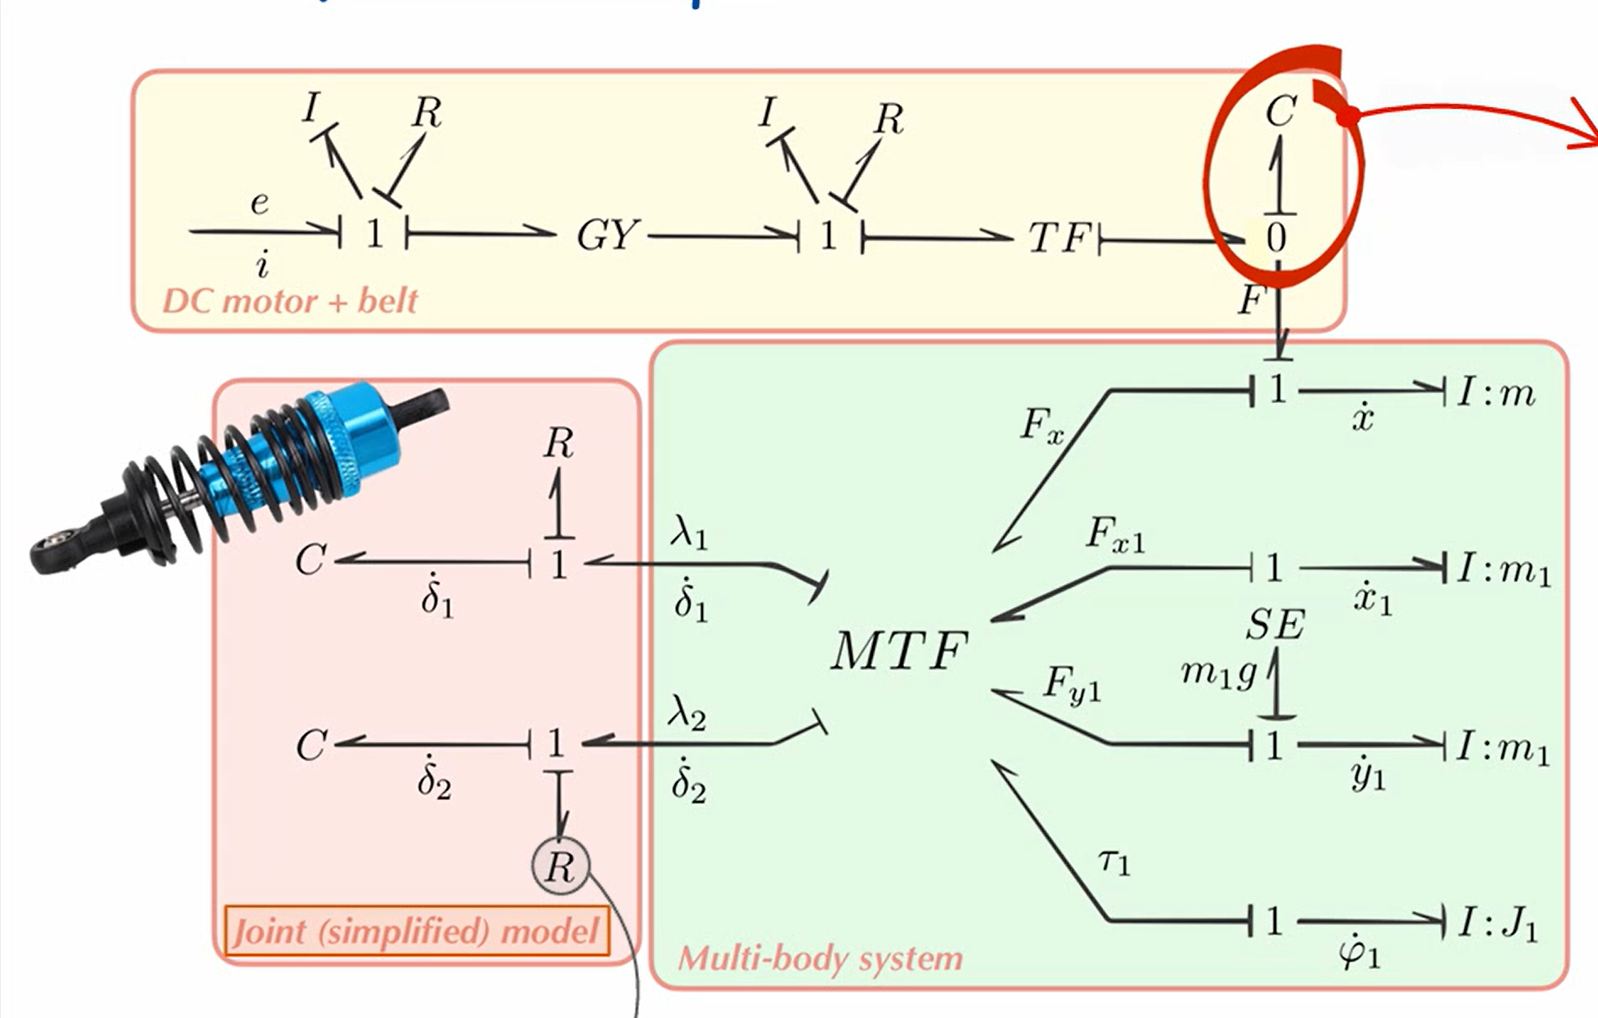
\includegraphics[width=0.8\textwidth]{figs/chapter6/6_14.png}
  \caption{Example of RC simplified model for joint}
\end{figure}



\section{Lagrangian mechanics and IC-fields (D.A.M.)}

The combination of I-fields (kinetic energy) and C-fields (potential energy) in a bond graph with a junction structure encoding kinematic constraints is exactly equivalent to a Lagrangian description. 

If we have a holonomic, lagrange-regular mechanical system, the kinetic energy is a quadratic-affine form: $T = \frac{1}{2}\dot{\mathbf{q}}_k^T \mathbf{M}(\mathbf{q}_k)\dot{\mathbf{q}}_k + \dot{\mathbf{q}}_k^T \mathbf{a}(\mathbf{q}_k)$. 
If $\mathbf{q}_k$ are generalised coordinates, then the Lagrange equations:
\begin{equation}
  \frac{d}{dt}\frac{\partial T}{\partial \dot{q}_i} - \frac{\partial T}{\partial q_i} = E_i
\end{equation}
(where $E_i$ includes potential energy derivatives and external forces) are automatically encoded by the bond graph. The IC-field representation makes this connection explicit and is particularly useful for systems with many degrees of freedom where writing Lagrange equations by hand is error-prone.

It's possible to write the Lagrangian Equations into Hamiltonian equations by the following formulas:

\begin{align}
  p_i = \frac{\partial T}{\dot{q}_i} \\
  \dot{p}_i = \frac{\partial T}{q_i} + E_i \\
\end{align}

where $E_i$ are the generalized forces

The first relation has always a special form:

$$
p_k = M(q_k, t) \dot{q}_k + a(q_k, t)
$$

Therefore we can write: 

$$
\dot{q}_k = M^{-1}(q_k, t) \[p_k - a(q_k, t)
$$

\begin{figure} [H]
  \centering
  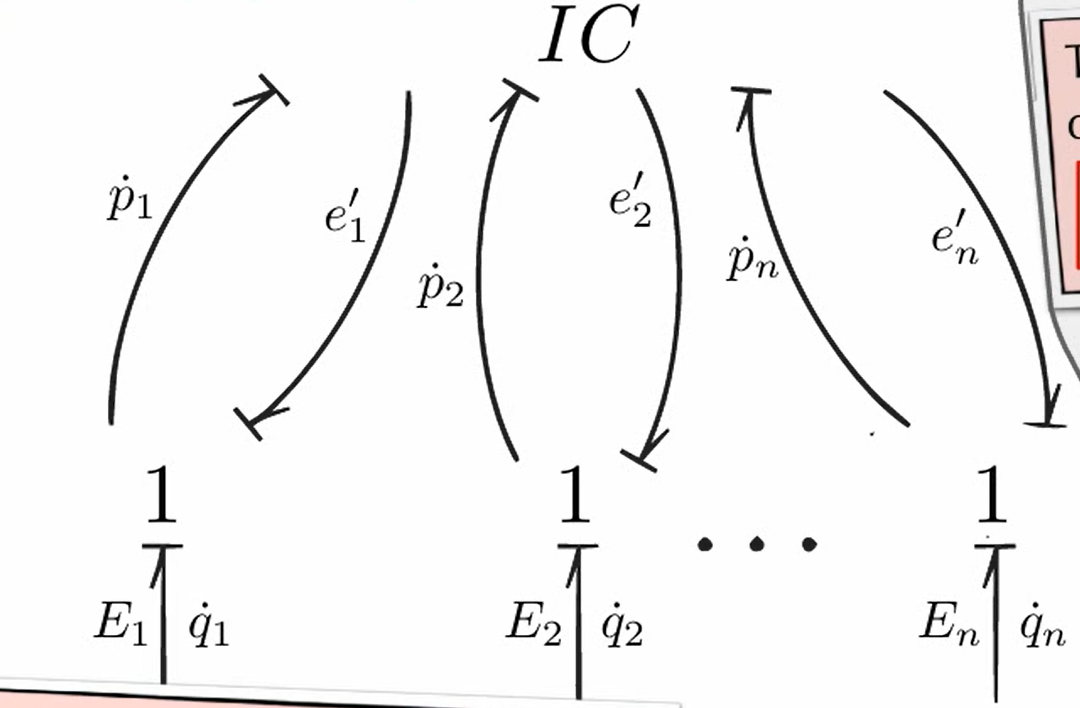
\includegraphics[width=0.8\textwidth]{figs/chapter6/6_15.png}
  \caption{IC field representing the Hamiltonian form of Lagrangian equations}
\end{figure}



\paragraph{The Hamiltonian Form and the D.A.M.}
The \textbf{Dynamic Analysis Method (D.A.M.)} replaces the kinematic junction structure with a true dynamic IC-field based on Hamilton's equations. The Hamiltonian is defined as $\mathcal{H} = \mathbf{p}_k^T\dot{\mathbf{q}}_k - \mathcal{L}$. By defining generalised momenta $\mathbf{p}_k = \partial T / \partial \dot{\mathbf{q}}_k$, we can invert the mass matrix to find velocities:

In the bond graph, the IC-field acts with an I-part computing $\dot{\mathbf{q}}_k$ (flows) from $\mathbf{p}_k$ (momenta), and a C-part computing the internal efforts $\mathbf{e}'_k$ from $\mathbf{q}_k$ (displacements). 

The \emph{main advantage} of this Hamiltonian IC-field approach is that it mathematically guarantees integral causality everywhere, avoiding algebraic loops entirely. The \emph{major drawback} is that the configuration-dependent mass matrix $\mathbf{M}(\mathbf{q}_k, t)$ must be non-singular and continuously inverted during the simulation.